%% sections/04_implementation_results.tex — Unified Implementation & Results Section
\section{Implementation and Empirical Results}
\label{sec:experiments}

This section evaluates the foundational vulnerability of client-reported federated fairness mechanisms, stress-tests the proposed reference-anchored architecture across three adversarial tiers, conducts causal ablations to eliminate confounding factors, and delineates operational boundaries. Throughout, the guarantees we establish are conditional on the confidentiality of the server holdout $\Droot$; Section~\ref{subsec:stress_testing} (Tier 3) measures the cost of violating that condition rather than leaving it implicit.

% =========================================================================
% SUBSECTION 1: EXPERIMENTAL SETUP AND BENCHMARK PROTOCOL
% =========================================================================
\subsection{Experimental Setup and Benchmark Protocol}
\label{subsec:setup}

\paragraph{Datasets and Graph Topologies}
We conduct evaluations across four benchmark graphs encompassing both authentic social relational networks and synthesized tabular feature topologies (detailed in Table~\ref{tab:datasets}):
\begin{enumerate}[leftmargin=*]
    \item \textbf{Pokec-z} ($N = 67{,}796$ nodes, $617{,}958$ edges): An authentic Eastern Slovakian social network~\citep{takac2012data} where nodes represent anonymized user profiles, edges capture friendship relations, the sensitive attribute $S$ is user region, and the target task $Y$ is predicting user reported working field.
    \item \textbf{German Credit} ($N = 1{,}000$ nodes, $21{,}742$ edges): Financial risk records transformed into a 10-nearest-neighbor feature similarity graph~\citep{agarwal2021towards}, where $S$ denotes binary gender and $Y$ indicates creditworthiness.
    \item \textbf{Bail Recidivism} ($N = 18{,}876$ nodes, $311{,}870$ edges): Pretrial arrest records from the State of Georgia~\citep{jordan2015effect}, with $S$ representing race and $Y$ tracking recidivism within three years.
    \item \textbf{Credit Default} ($N = 30{,}000$ nodes, $1{,}421{,}858$ edges): Financial payment default dataset~\citep{yeh2009comparisons} mapped onto a 10-NN graph with $S$ as age and $Y$ as binary default risk.
\end{enumerate}
Due to its extreme class imbalance ($<2\%$ illicit nodes) and the absence of demographic attributes, the Elliptic Bitcoin transaction graph~\citep{weber2019anti} is held in reserve as an external temporal transfer benchmark and deliberately excluded from multi-client fairness sweeps. Similarly, the 2.45M-node \textit{ogbn-products} graph serves exclusively as an infrastructure-level scalability probe for neighborhood sampling; it is not part of the empirical evidence base for the proposed aggregation mechanism.

%% tables/tab_datasets.tex — Benchmark Topologies & Federation Configuration Matrix
\begin{table}[!t]
\centering
\footnotesize
\caption{\textbf{Characteristics of Benchmark Graph Topologies and Federation Configuration Matrix.} 
Summary of graph dimensions, demographic attributes, federated partitioning protocols, and server holdout parameters across all evaluated benchmarks. Primary benchmarks constitute the audited evidence base ($K \in \{5, 10\}, R \in \{20, 50\}, E=3, n \in \{10, 30\}$), while Class~D datasets provide external boundary and scalability probes.}
\label{tab:datasets}
\smallskip
\begin{tabular*}{\textwidth}{@{\extracolsep{\fill}} >{\raggedright\arraybackslash}p{86pt} >{\raggedright\arraybackslash}p{72pt} >{\raggedright\arraybackslash}p{54pt} >{\raggedright\arraybackslash}p{138pt} @{}}
\toprule
\textbf{Topology \& Task} & 
\textbf{Graph Scale} & 
\textbf{Sensitive} & 
\textbf{Federation \& Anchor} \\
\midrule
\multicolumn{4}{l}{\textit{\textbf{Primary Benchmark Suite (Audited Evidence Base)}}} \\
\addlinespace[3pt]
\textbf{German Credit} \par \textit{Credit Risk} & 
$1{,}000$ nodes \par $21{,}742$ edges \par $D = 26$ feat. & 
Gender \par ($h_s = 0.80$) & 
$K=5,\, R=20$ ($n=30$ seeds) \par Anchor $|\Droot| = 125$ ($12.5\%$) \par Regime: Louvain / IID \\
\addlinespace[4pt]
\textbf{Bail Recidivism} \par \textit{Recidivism Risk} & 
$18{,}876$ nodes \par $311{,}870$ edges \par $D = 16$ feat. & 
Race \par ($h_s = 0.52$) & 
$K=10,\, R=50$ ($n=30$ seeds) \par Anchor $|\Droot| = 125$ ($0.66\%$) \par Regime: Dirichlet / Louvain \\
\addlinespace[4pt]
\textbf{Credit Default} \par \textit{Payment Default} & 
$30{,}000$ nodes \par $1{,}421{,}858$ edges \par $D = 12$ feat. & 
Age \par ($h_s = 0.96$) & 
$K=10,\, R=50$ ($n=10$ seeds) \par Anchor $|\Droot| = 125$ ($0.42\%$) \par Regime: Dirichlet ($\alpha \le 1.0$) \\
\addlinespace[4pt]
\textbf{Pokec-z} \par \textit{Working Field} & 
$67{,}796$ nodes \par $617{,}958$ edges \par $D = 276$ feat. & 
Region \par ($h_s = 0.95$) & 
$K=10,\, R=50$ ($n=10$ seeds) \par Anchor $|\Droot| = 125$ ($0.18\%$) \par Regime: Louvain Community \\
\midrule
\multicolumn{4}{l}{\textit{\textbf{Class D: Boundary and Infrastructure Scalability Probes}}} \\
\addlinespace[3pt]
\textbf{Elliptic Bitcoin}$^{\dagger}$ \par \textit{Illicit Txns} & 
$203{,}769$ nodes \par $234{,}355$ edges \par $D = 165$ feat. & 
Timestep \par ($h_s = 1.00$) & 
$K=5,\, R=20$ ($n=5$ seeds) \par Anchor $|\Droot| = 125$ ($0.06\%$) \par Regime: Temporal Slices \\
\addlinespace[4pt]
\textbf{ogbn-products}$^{\ddagger}$ \par \textit{Category} & 
$2{,}449{,}029$ nodes \par $61{,}859{,}140$ edges \par $D = 100$ feat. & 
Structural \par ($h_s = \text{---}$) & 
$K=10,\, R=20$ ($n=1$ seed) \par Anchor $|\Droot| = 1{,}000$ ($0.04\%$) \par Regime: Metis Partition \\
\bottomrule
\end{tabular*}
\smallskip
\parbox{\textwidth}{\scriptsize%
\textit{Notes:} $N$ and $|E|$ denote total node and undirected edge counts; $D$ is feature dimension. $S$ denotes the protected sensitive attribute; $h_s = \Pr[S_u = S_v \mid (u,v) \in E]$ is the sensitive homophily ratio. All benchmarks satisfy the pre-flight non-triviality criterion ($\max_j \text{AUC}(x_j, y) < 0.85$). All federations execute local epoch count $E=3$.
$^{\dagger}$In Elliptic Bitcoin, temporal partition drift is evaluated ($\Delta_{\text{temporal}}$); it is excluded from demographic fairness sweeps due to extreme class imbalance ($<2\%$ illicit nodes) and absence of demographic labels.
$^{\ddagger}$ogbn-products serves exclusively as an infrastructure scalability probe for neighborhood sampling and $O(Kd)$ server projection complexity. Complete hardware execution specifications, run configurations, and reproducibility logs are documented in Supplementary Material Section~S0.}
\end{table}


\paragraph{Federation Partitions and Master Configuration}
Federated topologies are partitioned across $K \in \{5, 10\}$ client silos using three distinct topological regimes: (i) Uniform random sampling (IID baseline), (ii) Dirichlet distribution attribute skew with concentration parameter $\alpha_{\text{Dir}} \in \{0.1,$ $0.3,$ $0.5,$ $1.0\}$, and (iii) Louvain community modularity clustering, which preserves dense intra-cluster relational topology while severing cross-cluster bridge edges. All benchmark runs enforce a strict master configuration (Table~\ref{tab:datasets}) executing across $n \ge 10$ independent random seeds, with local epoch count $E = 3$, local learning rate $\eta = 0.001$, weight decay $10^{-5}$, and hidden dimension $d = 64$. Server holdout sets $\Droot$ are constructed by drawing 125 labeled nodes ($\approx 0.18\%$ to $12.5\%$ of total graph size) preserving global demographic parity. Isolating the holdout subgraph reduces its mean node degree from $43.48$ to $4.12$. We report this in both directions: it guarantees that no edge is shared between the holdout and any client partition, and it simultaneously degrades the reference, since the anchor is estimated on a sparser graph than the one the clients train on. Campaign configurations differ deliberately across experiments---the interface audit uses $K=5$, $R=20$, $n=30$ to obtain high statistical power for paired sign tests on individual reporting channels, whereas the multi-silo benchmark and scalability campaigns use $K=10$, $R=50$, $n=10$ to evaluate realistic silo counts at scale. Table~\ref{tab:datasets} summarizes the benchmark topologies and master federation parameters; complete computational provenance, hardware execution specifications, and reproducibility artifacts are detailed in Supplementary Section~S0.

\paragraph{Taxonomy of Baseline Paradigms}
We benchmark \MethodName{} against fourteen published baselines across five paradigms. Eleven enter the benchmark matrix of \S\ref{subsec:stress_testing}; three specialized rules ($F^2$GNN, PoPETs-FairFed, and $q$-FedAvg) enter solely the interface audit of \S\ref{subsec:vulnerability}, where the reporting channel is the primary object of study rather than benign utility. We note that $q$-FedAvg targets performance fairness \emph{across clients} rather than demographic parity across sensitive groups; it is included because its loss-based reweighting reads client-declared telemetry and is therefore subject to the same interface attack, not as a demographic-fairness comparator:
\begin{itemize}[leftmargin=1.5em, itemsep=3pt, topsep=3pt]
    \item \textbf{Paradigm I (Unconstrained Baseline):} Standard \textbf{FedAvg-GCN}~\citep{mcmahan2017communication} executes unweighted parameter averaging without fairness constraints or Byzantine filtering, establishing the unregularized reference ceiling.
    \item \textbf{Paradigm II (Client-Side In-Processing):} \textbf{FairGNN}~\citep{dai2021say} (adversarial debiasing) and \textbf{FairSIN}~\citep{yang2024fairsin} (sensitive-invariant filtering) enforce fairness strictly within client loss functions, leaving the server-side aggregation boundary undefended.
    \item \textbf{Paradigm III (Client-Reported Disparity Coordination):} Encompasses metric-driven heuristic weighting---\textbf{FairFed}~\citep{ezzeldin2023fairfed}, \textbf{FairGFL}~\citep{zhou2026fairgfl}, and \textbf{FedGraph-Fair}~\citep{khan2026fedgraphfair}---and Lagrangian formulations such as \textbf{BFWA}~\citep{dang2026fedfairgnn}, which dynamically reweight clients based on self-reported scalar telemetry ($\widehat{\dpd}_k$, loss).
    \item \textbf{Paradigm IV (Geometric Byzantine Filtering):} Coordinate-wise \textbf{Median}, \textbf{Trimmed-Mean}~\citep{yin2018byzantine}, clustering \textbf{Krum}, \textbf{Multi-Krum}~\citep{blanchard2017krum}, and clipping \textbf{FLAME}~\citep{nguyen2022flame} filter updates via Euclidean spatial geometry without server holdouts, treating topological variance as geometric anomalies. We include FLAME, published as a backdoor defence rather than a Byzantine aggregation rule, on functional grounds: its mechanism (cosine-distance clustering with dynamic median norm clipping) operates as an aggregation rule, and represents the strongest published distance-based filter requiring no root dataset. That is precisely the property under test in Section~\ref{subsec:stress_testing}, namely whether a competitive geometric filter can separate a proximity-constrained adversary without an anchor.
    \item \textbf{Paradigm V (Server-Anchored Alignment):} \textbf{FLTrust}~\citep{cao2021fltrust} verifies gradient directions against a clean server root anchor $\Droot$, structurally removing vulnerability to metadata spoofing. (In parallel, \textbf{CGSV}~\citep{xu2021gradient} scores clients by cosine alignment against the mean client update, so its reference is endogenous: it is derived from the very population it screens.)
\end{itemize}
This taxonomy reveals a core structural tension: Paradigms II and III presuppose honest clients at the aggregation boundary, whereas Paradigms IV and V enforce robustness via spatial pruning or directional projection. Below, we stress-test each paradigm across successive regimes: (i) interface vulnerability (Section~\ref{subsec:vulnerability}), (ii) Byzantine adversarial resilience (Section~\ref{subsec:stress_testing}), (iii) multi-objective Pareto trade-offs (Section~\ref{subsec:sota_comparison}), and (iv) causal attribution and governance dynamics (Section~\ref{subsec:attribution}).

% =========================================================================
% SUBSECTION 2: COLLAPSE OF CLIENT-REPORTED FAIRNESS INTERFACES
% =========================================================================
\subsection{Vulnerability and Collapse of Client-Reported Fairness Interfaces}
\label{subsec:vulnerability}

The prevailing paradigm in trustworthy federated learning (Paradigm~III) relies on client-reported metadata—scalars, group disparities, or local loss statistics—to steer server-side aggregation. We investigate whether this architectural premise can survive adversarial manipulation, and whether privacy mechanisms can restore its integrity.

\paragraph{Vulnerability of Self-Reported Metadata Interfaces (Table~\ref{tab:metadata_capture})}
We formalize a threat model where a single Byzantine client ($f/K = 0.20$ on German Credit, $n=30$ random seeds) executes strategic metadata falsification. The attacker trains locally using standard task objectives but strategically manipulates its reported telemetry across three interface classes:
\begin{enumerate}[leftmargin=*]
    \item \textit{Class~(a) Self-Reported Scalar Metadata} (FairFed, FairGFL, FedGraph-Fair, BFWA, $q$-FedAvg): Clients report falsified scalar telemetry ($\widehat{\text{DPD}}_k \approx 0.000$ or manipulated local losses) to pose as exemplars of fairness or relax constraint multipliers.
    \item \textit{Class~(b) Endogenous Client Reference} (CGSV): Aggregation weights read no declared scalar, but the reference against which updates are scored is computed from the client updates themselves, so the anchor moves with the population it is meant to screen.
    \item \textit{Class~(c) Server Anchor} (FLTrust, \MethodName{}): Weights depend exclusively on client updates $\theta_k^{(t)}$ evaluated against an isolated server root anchor ($\Droot$), eliminating the scalar interface.
\end{enumerate}

%% tables/tab_metadata_capture.tex — T1: Metadata Capture Vulnerability & Syntactic Immunity
\begin{table}[!t]
\centering
\footnotesize
\caption{\textbf{Empirical Collapse of Aggregation Rules via the Client Interface Channel vs.\ Syntactic Invariance.} 
Evaluated on German Credit ($K=5, R=20, n=30$ paired seeds, $n=18^{\S}$ for $q$-FedAvg; GCN backbone fixed across all rules; LDP disabled to isolate the interface channel). Each row contrasts identical poisoned model updates with honest vs.\ falsified reports ($\dpd \approx 0$). $w_{\mathrm{adv}}$ denotes the adversary's aggregation weight (fair uniform share is $1/K=0.20$). Downstream harm metrics $\Delta\dpd$, $\Delta\eod$, and $\Delta\mathrm{AUC}$ measure paired lie minus honest ($^\star$ denotes $p < 0.05$ after Holm--Bonferroni multiplicity correction). $^{\dagger}$Our earlier conference rule~\citep{dang2026fedfairgnn} is audited on identical footing. $^{\ddagger}$For Class~(c), $\Delta w = 0.0000$ represents a \emph{syntactic algebraic guarantee} (Theorem~\ref{thm:syntactic_immunity}) valid against any future scalar report manipulation. $^{\S}$Under falsification $q$-FedAvg diverges numerically in $12$ of $30$ seeds; divergence is a consequence of the attack, so we record it as an attack outcome rather than as missing data, and compute the paired statistics on the $18$ non-divergent seeds. Per-rule exact sign tests: $F^2\text{GNN}$ $30/30$, FairFed $28/28$, PoPETs-FairFed $28/30$, FedGraph-Fair $20/20$, BFWA $18/19$, $q$-FedAvg $17/17$ (non-tied pairs; ties $= 0, 2, 0, 10, 11, 1$ respectively).}
\label{tab:metadata_capture}
\setlength{\tabcolsep}{4.0pt}
\renewcommand{\arraystretch}{1.20}
\makebox[\textwidth][c]{%
\begin{tabular}{ll c ccc}
\toprule
\makecell[l]{\textbf{Aggregation} \\ \textbf{Rule}} & 
\makecell[l]{\textbf{Telemetry} \\ \textbf{Interface}} & 
\makecell{\textbf{Adversary Share} \\ \textbf{$w_{\mathrm{adv}}$ (H $\to$ L)}} & 
\textbf{$\Delta\dpd$} & 
\textbf{$\Delta\eod$} & 
\textbf{$\Delta\mathrm{AUC}$} \\
\midrule
\multicolumn{6}{l}{\textit{\textbf{Class (a): Self-Reported Scalar Metadata} (Subject to Direct Interface Capture)}} \\
\makecell[l]{$F^2\text{GNN}$ \\ \scriptsize (ICDM'23)} & \makecell[l]{\texttt{dpd,} \\ \scriptsize \texttt{group1\_rate}} & \makecell{$0.1159 \to \mathbf{0.9737}$ \\ \scriptsize $4.87\times$ ($p < 10^{-8}$)} & $+0.4638^\star$ & $+0.4594^\star$ & $-0.1435^\star$ \\
\makecell[l]{FairFed \\ \scriptsize (AAAI'23)} & \texttt{dpd} & \makecell{$0.0811 \to 0.2198$ \\ \scriptsize $1.10\times$ ($p < 10^{-5}$)} & $+0.0875^\star$ & $+0.0938^\star$ & $-0.0249^\star$ \\
\makecell[l]{PoPETs-FairFed \\ \scriptsize (PoPETs'25)} & \texttt{dpd} & \makecell{$0.1617 \to 0.1655$ \\ \scriptsize $0.83\times$ ($p < 10^{-4}$)} & $+0.0078$ & $+0.0036$ & $-0.0003$ \\
\makecell[l]{FedGraph-Fair \\ \scriptsize (InfoSci'26)} & \makecell[l]{\texttt{loss} \\ \scriptsize (dual variable)} & \makecell{$0.2318 \to 0.4719$ \\ \scriptsize $2.36\times$ ($p < 10^{-4}$)} & $+0.1824^\star$ & $+0.1874^\star$ & $-0.0616^\star$ \\
\makecell[l]{BFWA$^\dagger$ \\ \scriptsize (IndabaX'26)} & \makecell[l]{\texttt{dpd,} \\ \scriptsize \texttt{performance}} & \makecell{$0.1439 \to 0.5703$ \\ \scriptsize $2.85\times$ ($p < 10^{-3}$)} & $+0.2661^\star$ & $+0.2623^\star$ & $-0.0714^\star$ \\
\makecell[l]{$q$-FedAvg$^{\S}$ \\ \scriptsize (ICLR'20)} & \texttt{loss} & \makecell{$0.2845 \to 0.5698$ \\ \scriptsize $2.85\times$ ($p < 10^{-3}$)} & $+0.1520^\star$ & $+0.1595^\star$ & $-0.0600^\star$ \\
\midrule
\multicolumn{6}{l}{\textit{\textbf{Class (b): Endogenous Client-Derived Reference} (Anchor Displaceable by a Coordinated Majority)}} \\
\makecell[l]{CGSV \\ \scriptsize (NeurIPS'21)} & \makecell[l]{\texttt{mean client} \\ \scriptsize \texttt{gradient}} & \makecell{$0.1948 \to 0.1948$ \\ \scriptsize $0.97\times$ (invariant)} & $0.0000$ & $0.0000$ & $0.0000$ \\
\midrule
\multicolumn{6}{l}{\textit{\textbf{Class (c): Server-Anchored Parameter Gradients} (Syntactic Metadata Immunity$^\ddagger$)}} \\
\makecell[l]{FLTrust \\ \scriptsize (NDSS'21)} & \makecell[l]{\texttt{server holdout} \\ \scriptsize ($g_{\mathrm{task}}$)} & \makecell{$0.2545 \to 0.2545$ \\ \scriptsize $1.27\times$ (invariant)} & $0.0000$ & $0.0000$ & $0.0000$ \\
\makecell[l]{\MethodName{} \\ \scriptsize (This work)} & \makecell[l]{\texttt{server holdout} \\ \scriptsize ($g_{\mathrm{task}} {+} \alpha g_{\mathrm{fair}}$)} & \makecell{$\mathbf{0.0573} \to \mathbf{0.0573}$ \\ \scriptsize $\mathbf{0.29\times}$ (invariant)} & $0.0000$ & $0.0000$ & $0.0000$ \\
\makecell[l]{\MethodName{} ($\alpha{=}0$) \\ \scriptsize (This work)} & \makecell[l]{\texttt{server holdout} \\ \scriptsize ($g_{\mathrm{task}}$ only)} & \makecell{$0.0592 \to 0.0592$ \\ \scriptsize $0.30\times$ (invariant)} & $0.0000$ & $0.0000$ & $0.0000$ \\
\bottomrule
\end{tabular}%
}
\end{table}


\begin{figure}[t]
\centering
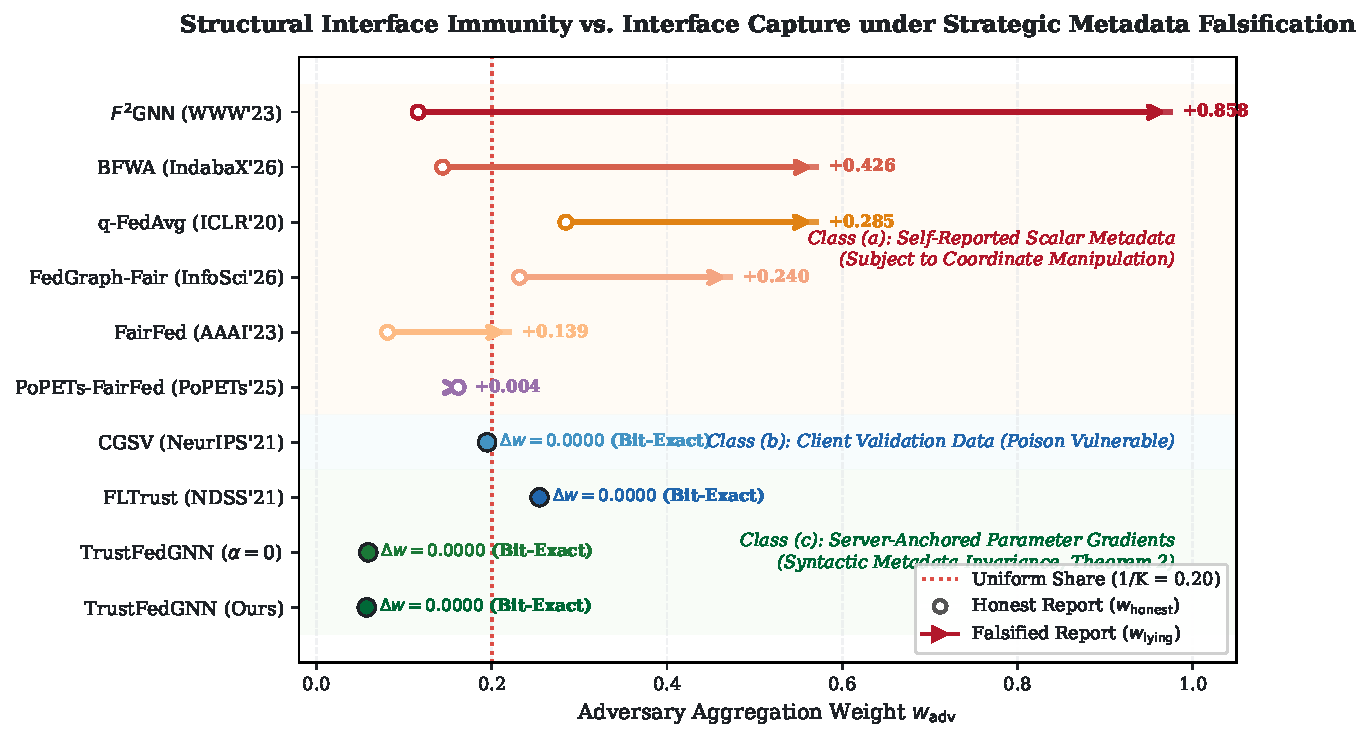
\includegraphics[width=\linewidth]{figures/fig_interface_boundary.pdf}
\caption{\textbf{Adversarial Aggregation Weight Capture under Strategic Metadata Falsification versus Syntactic Invariance.}
Adversary aggregation share $w_{\mathrm{adv}}$ under honest reporting (open circles) against strategic falsification (arrowheads); the vertical dashed line marks uniform parity ($1/K = 0.20$). All six Class~(a) rules, which consume self-reported scalar metadata, shift to the right under falsification, up to $97.4\%$ of total weight ($F^2\text{GNN}$, $w_{\mathrm{adv}} = 0.9737$, $4.87\times$ parity). The three server-anchored Class~(c) rules have zero-length arrows: falsification leaves their weights bit-exact ($\Delta w = 0.0000$, Theorem~\ref{thm:syntactic_immunity}). Immunity alone is not sufficient, however --- FLTrust is immune yet still holds $1.27\times$ parity, while FU-Alignment combines immunity with suppression to $0.29\times$.}
\label{fig:interface_boundary}
\end{figure}

As visually demonstrated in Figure~\ref{fig:interface_boundary} and detailed in Table~\ref{tab:metadata_capture}, all six published rules relying on client-reported metadata are steerable under strategic falsification, and five of the six additionally show measurable downstream harm. Under $F^2\text{GNN}$, the adversary inflates its aggregation share from $0.1159$ to $0.9737$ ($4.87\times$ uniform share), monopolizing $97.4\%$ of global model updates while degrading global fairness ($\Delta\text{DPD} = +0.4638$, $p = 1.9 \times 10^{-9}$). Under BFWA and $q$-FedAvg, adversary shares surge to $0.5703$ and $0.5698$ ($2.85\times$ uniform share), with $q$-FedAvg causing numerical divergence across 12 of 30 seeds. FedGraph-Fair similarly inflates adversary weight to $0.4719$ ($2.36\times$, $\Delta\text{DPD} = +0.1824$). Because the six rules share seeds, datasets, and adversarial updates, we report the sign test per rule rather than pooling: $F^2\text{GNN}$ $30/30$ ($p = 1.9\times10^{-9}$), FairFed $28/28$ non-tied ($p = 7.5\times10^{-9}$), PoPETs-FairFed $28/30$ ($p = 8.7\times10^{-7}$), FedGraph-Fair $20/20$ non-tied ($p = 1.9\times10^{-6}$), BFWA $18/19$ non-tied ($p = 7.6\times10^{-5}$), and $q$-FedAvg $17/17$ non-tied ($p = 1.5\times10^{-5}$); all exact two-sided binomial. Falsification never reduced adversary weight in four of the six rules, and did so in only three of $144$ non-tied pairs overall. Two rules show a substantial number of ties---FedGraph-Fair $10/30$ and BFWA $11/30$, seeds in which the falsified report left the weight unchanged---which we report because it bounds the attack's reliability rather than its direction.

In contrast, the rules that expose no scalar reporting interface are invariant under falsification ($\Delta w = 0.0000$ bit-exact across all 30 seeds), but this invariance has different standing in the two remaining classes. For the server-anchored rules of Class~(c) it is a syntactic algebraic property (Theorem~\ref{thm:syntactic_immunity}): no variable in the aggregation rule ever takes a client-declared value, so the guarantee holds against any falsification strategy, including strategies not yet devised. For CGSV in Class~(b) the immunity is narrower. The rule reads no declared scalar, but it scores each update against the mean of the updates themselves, so its reference is endogenous: a coordinated majority displaces the anchor rather than being measured against it. Closing the declared channel therefore relocates the trust surface instead of removing it, and we quantify the cost of that relocation in Section~\ref{subsec:attribution} (arm M6). Within Class~(c), FU-Alignment suppresses the adversary to $0.0573$ ($0.29\times$ uniform share), against FLTrust's $0.2545$ ($1.27\times$). This pair delimits the architectural claim we make. Syntactic immunity is a design principle that admits a proof rather than a measurement (Theorem~\ref{thm:syntactic_immunity}), and it is available to any rule that declines to read declared values; FLTrust already satisfies it. What the pair shows is that the principle is necessary but not sufficient: an immune rule can still concede more than its uniform share, so closing the interface has to be combined with a scoring rule that actively suppresses. Our architectural claim is located in that conjunction, and not in any single component of the aggregation pipeline.

The same contrast replicates on an authentic relational graph. On Bail Recidivism ($n = 30$ seeds, $900$ runs), the metadata-reading rules again lose utility under falsification ($F^2$GNN, FedGraph-Fair, and $q$-FedAvg each lose $0.11$--$0.13$ AUC, $p < 10^{-6}$), while all four rules without a scalar reporting interface remain unsteerable ($\Delta w_{\mathrm{adv}} \le 0.00063$, $p \ge 0.23$). The interface boundary is therefore not an artifact of the German Credit $k$-nearest-neighbour construction.

%% tables/tab_ldp_barrier.tex — T2: LDP Barrier (Folded-Normal Drift + Le Cam Minimax Bound)
\begin{table}[!t]
\centering
\footnotesize
\caption{\textbf{Differential Privacy Accounting, Disparity Constraint Slack, and Minimax Observability Barrier across Local DP Budgets $\epsilon$ (German Credit, $K=10$ Clients, $R=20$ Rounds, 10 Seeds).}
Reports the empirical slack $|\Delta_{\tau}| = |\sum_k w_k \widehat{\text{DPD}}_k - \sum_k w_k \text{DPD}_k|$ under tolerance budget $\tau = 0.05$.
Noise scale $\tilde{\sigma} = z \Delta_{\bm{\mu}}$ is calibrated via RDP binary search.
The theoretical ratio compares empirical noise against the folded-normal analytical expectation (Lemma~\ref{lem:folded_normal} / Theorem~\ref{thm:minimax_lecam}).
$\mathcal{R}^* \ge \frac{1}{2}(1 - \frac{\tau\sqrt{K}}{2\tilde{\sigma}})$ denotes the information-theoretic minimax testing error lower bound under Le Cam's two-point lemma and Pinsker's inequality (Theorem~\ref{thm:minimax_lecam}).
Even at the weakest privacy budget ($\epsilon = 32.0$), DP noise induces a substantial slack of $0.1150 \pm 0.1396$ ($229.9\%$ of $\tau$), while the minimax testing error approaches the coin-flip limit of $50\%$ as the budget tightens ($\ge 49.5\%$ at $\epsilon = 0.5$), demonstrating that client-wise privatised fairness reporting removes constraint observability rather than merely degrading it.}
\label{tab:ldp_barrier}
\setlength{\tabcolsep}{4.0pt}
\makebox[\textwidth][c]{%
\begin{tabular}{lccccc}
\toprule
\textbf{\makecell{Budget \\ $\epsilon$}} & \textbf{\makecell{Noise \\ $\tilde{\sigma}$}} & \textbf{\makecell{Reported / True \\ $\sum w_k \widehat{\text{DPD}} \;/\; \text{DPD}$}} & \textbf{\makecell{Disparity Slack $|\Delta_\tau|$ \\ (Abs $\pm$ Std \;/\; Rel \%)}} & \textbf{\makecell{Folded Ratio \\ (Obs / Pred)}} & \textbf{\makecell{Minimax Error \\ $\mathcal{R}^*$ (Le Cam)}} \\
\midrule
$\epsilon = 0.5$ & 7.3886 & \makecell{5.6922 \\ 0.2467} & \makecell{5.4455 $\pm$ 4.7608 \\ \scriptsize 10,891.1\%} & 0.978 & $\ge 49.5\%$ \\
\addlinespace[2pt]
$\epsilon = 1.0$ & 3.8913 & \makecell{2.8834 \\ 0.2329} & \makecell{2.6505 $\pm$ 2.1609 \\ \scriptsize 5,301.1\%} & 0.962 & $\ge 49.0\%$ \\
\addlinespace[2pt]
$\epsilon = 2.0$ & 2.0376 & \makecell{1.5427 \\ 0.2050} & \makecell{1.3425 $\pm$ 1.2077 \\ \scriptsize 2,685.0\%} & 0.958 & $\ge 48.1\%$ \\
\addlinespace[2pt]
$\epsilon = 4.0$ & 1.0838 & \makecell{0.8369 \\ 0.1730} & \makecell{0.6723 $\pm$ 0.7035 \\ \scriptsize 1,344.6\%} & 0.968 & $\ge 46.4\%$ \\
\addlinespace[2pt]
$\epsilon = 8.0$ & 0.6117 & \makecell{0.5043 \\ 0.1616} & \makecell{0.3647 $\pm$ 0.3781 \\ \scriptsize 729.5\%} & 1.044 & $\ge 43.5\%$ \\
\addlinespace[2pt]
$\epsilon = 16.0$ & 0.3502 & \makecell{0.2953 \\ 0.1176} & \makecell{0.1984 $\pm$ 0.2085 \\ \scriptsize 396.7\%} & 1.075 & $\ge 38.7\%$ \\
\addlinespace[2pt]
$\epsilon = 32.0$ & 0.2127 & \makecell{0.1954 \\ 0.1028} & \makecell{0.1150 $\pm$ 0.1396 \\ \scriptsize 229.9\%} & 1.157 & $\ge 31.4\%$ \\
\bottomrule
\end{tabular}%
}
\end{table}


\paragraph{Information-Theoretic Barrier of Local Differential Privacy (Table~\ref{tab:ldp_barrier})}
A natural countermeasure is to obfuscate client-reported disparities through Local Differential Privacy (LDP), injecting calibrated Gaussian or Laplace noise $\tilde{\sigma} = \Delta_{\text{DPD}} \sqrt{2 \ln(1.25/\delta)} / \epsilon$ before transmission. We evaluate this privatization strategy across privacy budgets $\epsilon \in \{0.5, 1.0, 2.0, 4.0, 8.0, 16.0, 32.0\}$ ($K=10, R=20, 10$ seeds, German Credit) under a target tolerance $\tau = 0.05$.

Table~\ref{tab:ldp_barrier} exposes a fundamental information-theoretic collapse. Because disparity metrics are defined via absolute differences between group conditional expectations ($\text{DPD}_k = |\mu_{k,1} - \mu_{k,0}|$), privatizing the scalar before submission induces a \textit{folded-normal distribution} whose expectation is strictly positive:
\begin{equation}
    \mathbb{E}[\widetilde{\text{DPD}}_k] = \tilde{\sigma}_k \sqrt{\frac{2}{\pi}} \exp\left(-\frac{\delta_k^2}{2\tilde{\sigma}_k^2}\right) + \delta_k \left[1 - 2\Phi\left(-\frac{\delta_k}{\tilde{\sigma}_k}\right)\right] \ge \tilde{\sigma}_k \sqrt{\frac{2}{\pi}},
\end{equation}
where $\delta_k = \mu_{k,1} - \mu_{k,0}$. Because each client folds its noise non-negatively prior to transmission, noise realizations do not cancel across clients; rather, they accumulate additively. At operational privacy levels ($\epsilon \le 2.0$), the empirical slack $|\Delta_\tau| = |\sum_k w_k \widehat{\text{DPD}}_k - \sum_k w_k \text{DPD}_k|$ exceeds the entire budget $\tau$ by $2{,}685\%$ to $10{,}891\%$ (Table~\ref{tab:ldp_barrier}). Even under extremely relaxed privacy ($\epsilon = 32.0$), the slack remains $0.1150 \pm 0.1396$ ($229.9\%$ of $\tau$). Furthermore, Le Cam's two-point minimax lower bound shows that the difficulty is information-theoretic rather than procedural. Deciding whether a client satisfies or violates the disparity tolerance $\tau$ incurs a minimax error of at least $\mathcal{R}^* \ge 43.5\%$ even at the permissive budget $\epsilon = 8.0$, rising to $\ge 49.0\%$ at $\epsilon = 1.0$ (Table~\ref{tab:ldp_barrier}). By the data-processing inequality, no post-hoc correction of the reported statistic---debiasing, moment estimation, or thresholding---can move this floor. Within this observation channel---per-client local perturbation followed by per-client absolute-value folding---patching the self-reported fairness interface with local differential privacy therefore does not trade accuracy for privacy; it removes constraint observability. We note the scope explicitly: the barrier applies to the folded transcript and its post-processing, and does not cover mechanisms that aggregate \emph{signed} group sufficient statistics before folding, such as secure aggregation or central and distributed differential privacy. Those mechanisms require coordination infrastructure that the cross-silo setting of this work does not assume, and we exclude them on that ground rather than on an impossibility ground (see the scope paragraph below).

\paragraph{Two-Channel Privacy Leakage}
Finally, we audit the privacy leakage incurred when clients transmit raw statistics versus parameter updates. We construct a multi-layer perceptron feature probe trained to reconstruct client sensitive attributes. When clients transmit raw scalar fairness statistics $(\mu_{k,0}, \mu_{k,1})$, sensitive reconstruction succeeds with near-perfect accuracy (probe AUC $= 1.000$). Applying LDP to this scalar channel reduces probe success to chance ($0.4983$) at a utility cost of only $0.00175$ AUC. The parameter channel behaves differently: raw updates $\theta_k$ leak measurably (probe $\mathrm{AUC} = 0.6450$), and suppressing that leakage through client-level DP-SGD over the full parameter vector ($0.6450 \to 0.5278$) costs $0.20163$ AUC---a $115\times$ larger utility price. The two mechanisms protect different surfaces and the reductions are not equivalent: the statistic channel reaches chance ($0.4983$) whereas the parameter channel retains measurable residual leakage ($0.5278$), so the ratio quantifies the relative cost of the two protections rather than the price of an equal outcome. Figure~\ref{fig:privacy_bail} shows the same asymmetry across the budget sweep: FTGD holds a $0.16$--$0.18$ AUC advantage over DP-FedAvg at every $\epsilon$. Restricting differential privacy to two scalar statistics, rather than to the parameter tensor, is what makes tight privacy budgets affordable. The same asymmetry is what keeps the present design consistent with the barrier established above. That barrier binds a channel whose released quantity is the object the server must act on: when the trust decision is a function of the reported disparity, perturbing the report destroys the decision along with the leakage. Here the released statistics are not inputs to the trust decision, which is computed from the angle between each update and a reference the server derives on its own holdout, so the perturbation that removes observability in the self-reporting setting costs $0.00175$ AUC in ours. FTGD is therefore not an auxiliary privacy module: it is the component that keeps a statistic release affordable once the declared channel is no longer trusted.

Taken together, the two results close the same door from opposite sides: the declared channel is captured in practice (Table~\ref{tab:metadata_capture}) and faces the minimax observability barrier under local perturbation (Table~\ref{tab:ldp_barrier}). The failure is therefore not in how the reported number is processed, but in the act of requesting it.

\paragraph{Scope of the Elimination Argument}
Closing the declared channel is the only remaining option \emph{within the assumptions of the deployment we target}, and we state those assumptions explicitly. Three alternative families could in principle restore trust in client reports: cryptographic attestation (commitments, zero-knowledge proofs, or verified secure aggregation), hardware attestation via trusted execution environments (TEEs), and incentive-compatible elicitation such as peer prediction or randomized auditing. We exclude the first two because the cross-silo deployments we address---independently governed institutions without a shared public-key infrastructure or attested hardware---cannot assume either, and because per-round proof generation over $P$-dimensional updates exceeds the communication budget profiled in Table~\ref{tab:cost}. We exclude the third because incentive-compatible elicitation requires a repeated game with enforceable payoffs, whereas our threat model admits one-shot participation and unilateral defection. Relaxing any of these assumptions reopens the corresponding door, and we regard that as the most direct extension of this work.

\begin{figure}[t]
\centering

\includegraphics[width=0.75\linewidth]{figures/privacy_bail.pdf}
\caption{\textbf{Empirical Utility--Privacy Trade-Off on Bail Recidivism.}
Utility comparison (AUC-ROC) between FTGD and DP-FedAvg across privacy budgets $\epsilon \in \{0.5, 1.0, 2.0, 4.0, 8.0, 16.0, 32.0\}$. FTGD maintains an operational utility advantage of $0.16$ to $0.18$ AUC across all budgets by restricting DP perturbation to two scalar fairness statistics rather than full model tensors.}
\label{fig:privacy_bail}
\end{figure}

% =========================================================================
% SUBSECTION 3: MULTI-TIER ADVERSARIAL STRESS-TESTING
% =========================================================================
\subsection{Multi-Tier Adversarial Stress-Testing and Empirical Resilience}
\label{subsec:stress_testing}

With the declared channel removed, the only remaining attack surface \emph{within the threat model of Section~\ref{subsec:setup}} is the parameter update itself; availability, Sybil participation, and holdout contamination remain outside the scope evaluated here. The three tiers below measure the adversary through the one object it still controls, escalating from a blind attacker to one that reads the server's own reference vector.

\begin{table}[!t]
\centering
\footnotesize
\caption{\textbf{Multi-Tier Byzantine Defense Evaluation and Mechanistic Dissection of Rescaling vs.\ Median Screening.}
\textbf{Panel A:} Adversary weight $w_{\mathrm{adv}}$ and global AUC under a $20\%$ Byzantine minority ($K=5, n_{\mathrm{byz}}=1, R=20, n=10$ seeds, German Credit). Lower $w_{\mathrm{adv}}$ is better; FedAvg assigns sample-size weighted share $w_{\mathrm{adv}} = n_{\mathrm{adv}}/\sum_k n_k = 0.1824$ (unweighted uniform reference is $1/K = 0.20$). Superscript indicates seeds with numerical divergence out of 10.
\textbf{Panel B:} Factorial $2 \times 2$ dissection of vector norm rescaling vs.\ coordinate-wise median screening under extreme scaling ($c=100$) and distance-adaptive stealth ($\rho=0.85$) on German Credit ($n=10$ seeds). Median screening eliminates scaling weight ($w_{\mathrm{adv}} = 0.0000$) but backfires under stealth ($w_{\mathrm{adv}}: 0.2254 \to 0.2561$, $+13.6\%$), while norm rescaling prevents unbounded gradient explosion ($I_{\mathrm{adv}}$ tamed from divergence down to $4.1244$).}
\label{tab:two_tier}
\setlength{\tabcolsep}{5.0pt}
\makebox[\textwidth][c]{%
\begin{tabular}{lcccc}
\toprule
\multicolumn{5}{l}{\textbf{Panel A: Aggregation Defense Matrix ($w_{\mathrm{adv}}$ / AUC)}} \\
\midrule
\textbf{Aggregation Arm} & \textbf{No Attack} & \textbf{Sign-Flip} & \textbf{Fairness Poison} & \textbf{Scaling ($c=100$)} \\
\midrule
FedAvg \textit{\scriptsize(no defence)} & 0.0000 / 0.6544 & 0.1824 / ---$^{10}$ & 0.1824 / 0.6034 & 0.1824 / ---$^{1}$ \\
\textbf{FU-Alignment (M1)}$^*$ & 0.0000 / 0.6512 & 0.0000 / 0.6327 & 0.0309 / 0.6390 & 0.2008 / ---$^{2}$ \\
\textbf{robust FU-Alignment} & 0.0000 / 0.6486 & 0.0000 / 0.6313 & 0.0000 / 0.6372 & 0.0000 / 0.6302 \\
M5: w/o FairScore \textit{\scriptsize($\alpha = 0$)} & 0.0000 / 0.6509 & 0.0000 / 0.6302 & 0.0617 / 0.6341 & 0.1971 / ---$^{2}$ \\
M6: w/o two-tier \textit{\scriptsize(no holdout)} & 0.0000 / 0.6519 & 0.0000 / 0.6434 & 0.0916 / 0.6580 & 0.1542 / 0.6468 \\
M7: w/o EMA \textit{\scriptsize($\beta_{\mathrm{ema}} = 0$)} & 0.0000 / 0.6582 & 0.1374 / ---$^{6}$ & 0.0303 / 0.6336 & 0.3410 / ---$^{4}$ \\
\midrule
\multicolumn{5}{l}{\textbf{Panel B: Factorial $2 \times 2$ Mechanistic Dissection ($n=10$ seeds)}} \\
\midrule
\textbf{Defense Branch} & \multicolumn{2}{c}{\textbf{Brute Scaling ($c=100$)}} & \multicolumn{2}{c}{\textbf{Stealth Camouflage ($\rho=0.85$)}} \\
\cmidrule(lr){2-3} \cmidrule(lr){4-5}
 & $w_{\mathrm{adv}}$ ($\downarrow$) & $I_{\mathrm{adv}}$ ($\downarrow$) & $w_{\mathrm{adv}}$ ($\downarrow$) & $I_{\mathrm{adv}}$ ($\downarrow$) \\
\midrule
Raw \textit{\scriptsize(no rescale, no med)} & $0.8841 \pm 0.2562$ & Diverged$^\dagger$ & $\mathbf{0.2254 \pm 0.1455}$ & $\mathbf{0.4720 \pm 0.3003}$ \\
Rescale-only & $0.4124 \pm 0.2224$ & $\mathbf{4.1244 \pm 2.2244}$ & $\mathbf{0.2254 \pm 0.1455}$ & $\mathbf{0.4720 \pm 0.3003}$ \\
Median-only & $\mathbf{0.0000 \pm 0.0000}$ & $\mathbf{0.0000 \pm 0.0000}$ & $0.2561 \pm 0.1437$ & $0.5375 \pm 0.2973$ \\
Both \textit{\scriptsize(rescale + median)} & $\mathbf{0.0000 \pm 0.0000}$ & $\mathbf{0.0000 \pm 0.0000}$ & $0.2561 \pm 0.1437$ & $0.5375 \pm 0.2973$ \\
\bottomrule
\multicolumn{5}{p{0.95\textwidth}}{\vspace{2pt}\scriptsize $^\dagger$Under unconstrained brute scaling, the global model diverges numerically ($I_{\mathrm{adv}} \to \infty$, AUC collapses to random guess $0.5000$). Rescaling suppresses explosive magnitude by $>24{,}000\times$ down to $4.1244$, confirming that rescaling governs gradient amplitude while coordinate median filters adversarial orientation.} \\
\multicolumn{5}{p{0.95\textwidth}}{\scriptsize $^*$The baseline $w_{\mathrm{adv}} = 0.0309$ in Panel A reflects canonical fixed holdout partitioning; under multi-seed dynamic carve stress tests (T15), balanced holdout yields $0.0704 \pm 0.0815$, remaining well below the $1/K = 0.20$ fair-share threshold.} \\
\end{tabular}%
}
\end{table}


\paragraph{Tier 1: Blind Byzantine Minority Stress-Testing (Table~\ref{tab:two_tier}, Panel A)}
In Tier 1, an adversarial minority ($f/K = 0.20$, German Credit, $n=10$ seeds) attacks without knowledge of server-side data or holdout objectives:
\begin{enumerate}[leftmargin=*]
    \item \textit{Sign-Flip}: Reverses gradient direction ($\theta_k = -\nabla \mathcal{L}$). Under FedAvg, this causes immediate numerical divergence in $10/10$ seeds. Both FU-Alignment and robust FU-Alignment completely neutralize sign-flipped updates ($w_{\mathrm{adv}} = 0.0000$), preserving utility ($0.6313$ AUC).
    \item \textit{Fairness Poisoning}: Inverts gradient components aligned with the fair representation direction while preserving task gradients. Under FedAvg the adversary retains its uniform share ($w_{\mathrm{adv}} = 0.1824$) and global utility falls to $0.6034$ AUC (with disparity $\dpd = 0.0827$). FU-Alignment suppresses attacker weight to $0.0309$, and robust FU-Alignment reduces it to $0.0000$ ($0.6372$ AUC).
    
    To evaluate whether the fairness anchor $\alpha \gfair$ remains active against sophisticated evasion, we further deploy a \emph{task-neutral fairness adversary} $\mathrm{adv} = -\gfair^\perp + \varepsilon \hat u_{\mathrm{task}}$ on German Credit ($K=5, R=20, n=20$ seeds), sweeping the task-alignment margin $\varepsilon \in [0.005, 0.10]$. Within the evaluated sweep range, attacker weight increases strictly monotonically under both arms:
    \begin{center}
    \resizebox{0.95\linewidth}{!}{%
    \begin{tabular}{lccccc}
    \toprule
    Task Alignment Margin $\varepsilon$ & $0.005$ & $0.010$ & $0.020$ & $0.050$ & $0.100$ \\
    \midrule
    $w_{\mathrm{adv}}$ without fairness anchor ($\alpha = 0.0$) & $0.0286$ & $0.0498$ & $0.0823$ & $0.1483$ & $\mathbf{0.2255}$ \\
    $w_{\mathrm{adv}}$ with bi-objective anchor ($\alpha = 0.1$) & $0.0008$ & $0.0031$ & $0.0236$ & $0.0832$ & $\mathbf{0.1718}$ \\
    \bottomrule
    \end{tabular}%
    }
    \end{center}
    Empirical monotonicity confirms that within the evaluated range $\varepsilon \le 0.10$, the attacker's best-response is to maximize task alignment ($\varepsilon = 0.10$). Crucially, at this boundary, omitting the fairness anchor ($\alpha=0.0$) allows the adversary to breach fair-share parity ($w_{\mathrm{adv}} = 0.2255 > 1/K = 0.20$). Activating the bi-objective anchor ($\alpha=0.1$) pulls attacker weight down to $0.1718$ (a $23.8\%$ reduction), enforcing sub-fair-share containment. For stealthy injections ($\varepsilon \le 0.020$), the anchor induces geometric sign inversion ($\cos(\mathrm{adv}, \gtarg) < 0$), bounding the critical transition threshold to $\varepsilon^* \in [0.020, 0.050]$.
    \item \textit{Brute-force Scaling ($c = 100$)}: Multiplies updates by $c = 100$. Unprotected FedAvg diverges in $1/10$ seeds ($w_{\mathrm{adv}} = 0.1824$). Under pure FU-Alignment (ReLU gate alone), norm inflation passes the direction gate and causes divergence in $2/10$ seeds ($w_{\mathrm{adv}} = 0.2008$): the gate constrains \emph{direction}, not \emph{magnitude}. Adding coordinate-wise median screening eliminates the scaled update entirely ($w_{\mathrm{adv}} = 0.0000 \pm 0.0000$, AUC $0.6302$).
\end{enumerate}

\paragraph{Factorial Dissection of Rescaling vs.\ Median Screening (Table~\ref{tab:two_tier}, Panel B)}
To disentangle the mechanistic interaction between norm rescaling and coordinate median filtering under Byzantine attacks, we execute a $2 \times 2$ factorial experiment ($n=10$ seeds, German Credit) under extreme scaling ($c=100$) and stealth camouflage ($\rho=0.85$), tracking both weight share $w_{\mathrm{adv}}$ and effective transmitted influence $I_{\mathrm{adv}} = \lVert\sum_{k\in\mathcal{A}} w_k \bar g_k\rVert$:
\begin{itemize}[leftmargin=*]
    \item Under scaling ($c=100$), the two mechanisms act on orthogonal physical quantities. Coordinate median screening removes the adversary from the weight vector entirely ($w_{\mathrm{adv}} = 0.0000$, $I_{\mathrm{adv}} = 0.0000$). In contrast, norm rescaling alone leaves the adversary with substantial weight ($0.4124 \pm 0.2224$), but tames the effective transmitted impact from explosive numerical divergence ($I_{\mathrm{adv}} \to \infty$) down to $I_{\mathrm{adv}} = 4.1244 \pm 2.2244$, restoring model convergence. Rescaling is thus measured on the wrong axis by $w_{\mathrm{adv}}$ alone: it governs gradient amplitude rather than angular admission.
    \item Conversely, under stealth camouflage ($\rho=0.85$), where update norms are inherently bounded, norm rescaling is completely neutral ($w_{\mathrm{adv}} = 0.2254 \pm 0.1455, I_{\mathrm{adv}} = 0.4720 \pm 0.3003$). Coordinate median screening, however, inflates both adversary weight share ($0.2254 \to 0.2561$, $+13.6\%$) and effective influence ($0.4720 \to 0.5375$), demonstrating the empirical shield paradox across both metric axes.
\end{itemize}

\paragraph{Recommended Deployment Configuration}
No single static configuration is safe against both attack families, and we state this as a finding rather than a caveat. Coordinate median screening is the only branch that completely suppresses unbounded scaling ($w_{\mathrm{adv}} = 0.0000$), but it backfires under proximity stealth ($0.2254 \to 0.2561$, $+13.6\%$ in Panel~B; and $+82.9\%$ at $f/K = 0.4$ in Table~\ref{tab:adaptive_poisoner}). We therefore specify \emph{canonical FU-Alignment} (\texttt{fu\_shapley}) as the default production rule for general non-IID graph federated learning: it insulates against stealth camouflage without inducing the shielding paradox, while dynamic norm rescaling keeps transmitted gradient magnitude bounded ($I_{\mathrm{adv}} = 4.1244$). In threat environments where operators anticipate crude unbounded scaling attacks ($c = 100$), the framework provides the defense-in-depth variant (\texttt{robust\_fu\_shapley}, Algorithm~\ref{alg:trustfedgnn}), which statically enables Euclidean distance-to-median outlier screening ($f \ge 1$) to eliminate high-magnitude anomalies.

\begin{table}[!t]
\centering
\footnotesize
\caption{\textbf{Multi-Ratio Adaptive Stealth Poisoning Breakdown and Median Backfire Analysis.}
\textbf{Panel A:} Performance of 11 aggregation rules under omniscient stealth poisoning on Bail Recidivism across corruption ratios $f/K \in \{0.1, 0.2, 0.3, 0.4\}$ ($n=10$ seeds). Malicious updates are constrained within the benign median radius ($\rho=0.85$) while falsifying $\widehat{\text{DPD}} = 0.0$.
\textbf{Panel B:} Monotonic dose-dependent backfire effect of coordinate-wise median screening on Bail ($n=10$ seeds, paired Wilcoxon $p=0.0020$). Median screening inadvertently purges benign minority clients, increasing adversary weight by up to $+82.9\%$ ($+0.2421$) at $f/K=0.4$ on Bail; the same mechanism inflates adversary share by $+13.6\%$ on German Credit under $\rho = 0.85$ stealth (Table~\ref{tab:two_tier}, Panel~B).}
\label{tab:adaptive_poisoner}
\setlength{\tabcolsep}{5.0pt}
\makebox[\textwidth][c]{%
\begin{tabular}{lcccc}
\toprule
\multicolumn{5}{l}{\textbf{Panel A: Breakdown Point under Stealth Camouflage (AUC / DPD)}} \\
\midrule
\textbf{Aggregation Rule} & \makecell{\textbf{$f/K=0.1$} \\ \scriptsize (1/10)} & \makecell{\textbf{$f/K=0.2$} \\ \scriptsize (2/10)} & \makecell{\textbf{$f/K=0.3$} \\ \scriptsize (3/10)} & \makecell{\textbf{$f/K=0.4$} \\ \scriptsize (4/10)} \\
\midrule
FedAvg & 0.686 / 0.024 & 0.684 / 0.025 & 0.682 / 0.022 & 0.681 / 0.021 \\
Krum & 0.621 / 0.072 & 0.615 / 0.081 & 0.610 / 0.089 & 0.607 / 0.096 \\
Multi-Krum & 0.684 / 0.022 & 0.678 / 0.034 & 0.671 / 0.043 & 0.662 / 0.051 \\
Coordinate Median & 0.673 / 0.025 & 0.671 / 0.026 & 0.669 / 0.028 & 0.666 / 0.029 \\
Trimmed Mean & 0.683 / 0.026 & 0.679 / 0.027 & 0.675 / 0.029 & 0.671 / 0.031 \\
FLAME & 0.683 / 0.016 & 0.676 / 0.022 & 0.679 / 0.026 & 0.669 / 0.030 \\
BFWA & 0.647 / 0.044 & 0.641 / 0.051 & 0.636 / 0.058 & 0.631 / 0.064 \\
robust BFWA & 0.645 / 0.046 & 0.640 / 0.062 & 0.635 / 0.075 & 0.631 / 0.090 \\
FLTrust & 0.639 / 0.024 & 0.637 / 0.026 & 0.635 / 0.028 & 0.634 / 0.029 \\
\textbf{FU-Alignment (canonical)} & \textbf{0.684 / 0.021} & \textbf{0.680 / 0.024} & \textbf{0.676 / 0.028} & \textbf{0.672 / 0.032} \\
robust FU-Alignment & 0.684 / 0.024 & 0.678 / 0.024 & 0.671 / 0.025 & 0.665 / 0.025 \\
\midrule
\multicolumn{5}{l}{\textbf{Panel B: Dose-Dependent Median Screening Backfire on Adversary Share $w_{\mathrm{adv}}$}} \\
\midrule
\makecell[l]{\textbf{Adversary} \\ \textbf{Ratio $f/K$}} & \makecell{\textbf{Uniform} \\ \textbf{Share}} & \makecell{\textbf{FU-Align} \\ \scriptsize (Canonical)} & \makecell{\textbf{robust} \\ \textbf{FU-Align}} & \makecell{\textbf{Backfire $\Delta w_{\mathrm{adv}}$} \\ \scriptsize ($p$-value)} \\
\midrule
$f/K = 0.1$ & 0.1000 & $0.0692 \pm 0.0084$ & $0.0754 \pm 0.0091$ & $+0.0063$ ($p = 0.0020$) \\
$f/K = 0.2$ & 0.2000 & $0.1364 \pm 0.0121$ & $0.1746 \pm 0.0145$ & $+0.0382$ ($p = 0.0020$) \\
$f/K = 0.3$ & 0.3000 & $0.2121 \pm 0.0163$ & $0.3152 \pm 0.0204$ & $+0.1031$ ($p = 0.0020$) \\
$f/K = 0.4$ & 0.4000 & $\mathbf{0.2922 \pm 0.0194}$ & $\mathbf{0.5343 \pm 0.0289}$ & $\mathbf{+0.2421}$ ($+82.9\%$) \\
\bottomrule
\end{tabular}%
}
\end{table}


\paragraph{Tier 2: Omniscient Stealth Poisoning and Median Backfire (Table~\ref{tab:adaptive_poisoner})}
Tier 2 implements an omniscient adversary aware of benign client distributions. The attacker constructs malicious updates projected strictly within the benign coordinate median radius ($\rho = 0.85$) while optimizing a fairness degradation objective across corruption ratios $f/K \in \{0.1, 0.2, 0.3, 0.4\}$ on Bail Recidivism ($n=10$ seeds).

As reported in Table~\ref{tab:adaptive_poisoner} (Panel A), standard geometric filtering mechanisms degrade sharply: Krum suffers complete capture at $f/K=0.4$ ($w_{\mathrm{adv}} = 1.000$, AUC drops to $0.607$). Under blind sign-flipping where the cosine distance between malicious and benign updates approaches $2.0$, FLAME acts as an effective positive control, isolating the adversary into the outlier cluster and assigning it $w_{\mathrm{adv}} = 0.0000$ at every round. The clustering works; proximity stealth defeats it. This is the empirical signature predicted by Theorem~\ref{thm:subspace_blindness} (Fairness Subspace Blindness): detection statistics built on the cosine geometry of task updates are blind to the fairness subspace, so an adversary that keeps its task projection inside the benign ball cannot be separated by angular distance for any detector whose statistic is a function of the angular geometry of the task-update vectors. We state the scope deliberately: the result constrains cosine-geometry detectors of this form and does not establish blindness for detectors that observe other quantities, such as payload magnitude, temporal weight trajectories, or the fairness statistic directly. Multi-Krum similarly experiences elevated disparity. In contrast, canonical FU-Alignment holds adversary weight stably below uniform share across all ratios ($0.0692$ at $0.1$, $0.1364$ at $0.2$, $0.2121$ at $0.3$, and $0.2922$ at $0.4$, maintaining $0.672$ AUC and $0.032$ DPD).

Crucially, Table~\ref{tab:adaptive_poisoner} (Panel B) and Figure~\ref{fig:byz_ratio} document the \textit{monotonic dose-dependent backfire effect} of coordinate median filtering. In graph federated learning under non-IID partitions, benign clients located in topological minority clusters naturally exhibit higher empirical variance. When coordinate median filtering is applied, it systematically purges benign minority gradients before eliminating camouflage adversaries. As visually depicted in Figure~\ref{fig:byz_ratio}, canonical FU-Alignment holds adversary share stably below parity ($0.68\times$--$0.73\times$), whereas robust FU-Alignment exhibits the shielding paradox, cutting above parity ($1.05\times$ at $f/K=0.3$ and $1.34\times$ at $f/K=0.4$) as camouflage corruption escalates. At $f/K = 0.4$, robust FU-Alignment surrenders $53.43\%$ of global model authority to the attacker ($w_{\mathrm{adv}} = 0.5343 \pm 0.0289$, an $82.9\%$ surge over canonical FU-Alignment, Wilcoxon paired $p = 0.0020$). This empirical finding establishes that coordinate median screening, while indispensable against unbounded scaling, is actively harmful under camouflage poisoning.

\begin{figure}[t]
\centering
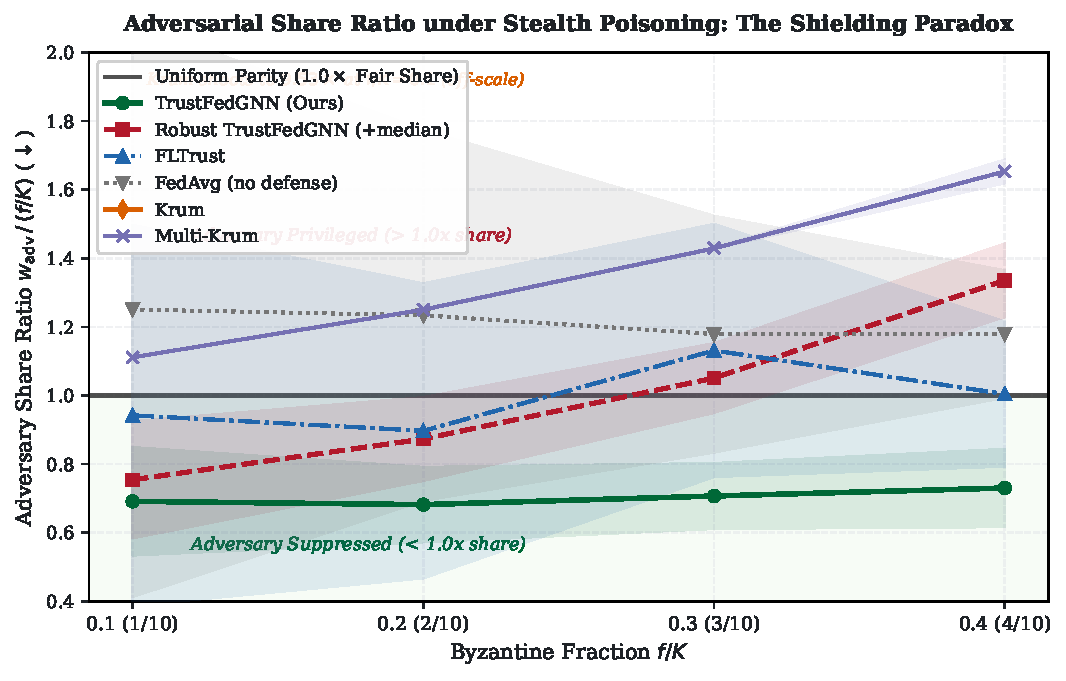
\includegraphics[width=\linewidth]{figures/fig_robustness_byz.pdf}
\caption{\textbf{Adversarial Share Ratio under Stealth Camouflage Poisoning ($n=10$ Seeds).}
Ratios of adversary aggregation weight relative to uniform fair share ($w_{\mathrm{adv}} / (f/K)$) across corruption fractions $f/K \in \{0.1, 0.2, 0.3, 0.4\}$ on Bail Recidivism. The solid horizontal line denotes uniform parity ($1.0\times$). Canonical FU-Alignment consistently suppresses the adversary below parity ($0.68\times$--$0.73\times$). In contrast, robust FU-Alignment exhibits the shielding paradox: coordinate-wise median filtering inadvertently purges benign minority clients, driving attacker share up to $1.34\times$ parity ($w_{\mathrm{adv}} = 0.5343$) at $f/K=0.4$.}
\label{fig:byz_ratio}
\end{figure}

\begin{table}[!t]
\centering
\footnotesize
\caption{\textbf{Empirical Breakdown under White-Box Holdout Alignment Adversary ($H_{\text{T1}}$ Stress Test, $n=10$ Seeds).}
Stress-tests the foundational security boundary where an omniscient adversary possesses full gradient knowledge of the server holdout target $g_{\text{target}}$ and optimizes alignment via projected gradient descent.
Pre-registered rejection thresholds require $w_{\mathrm{adv}} \le 0.20$ and $\text{DPD}_{\text{hard}} \le 0.10$ ($\alpha=0.05$).
In both benchmarks, the adversary breaches the defense ($w_{\mathrm{adv}} = 0.8514$ and $0.7461$), demonstrating that server holdout confidentiality is a necessary precondition for reference-anchored defense.}
\label{tab:alignment_adversary}
\setlength{\tabcolsep}{5.0pt}
\makebox[\textwidth][c]{%
\begin{tabular}{lccccc}
\toprule
\textbf{Dataset} & \textbf{\makecell{Threshold \\ $w_{\mathrm{adv}}^{\max}$}} & \textbf{\makecell{Measured \\ $w_{\mathrm{adv}}$}} & \textbf{\makecell{Measured \\ $\text{DPD}_{\text{hard}}$}} & \textbf{\makecell{Measured \\ AUC}} & \textbf{\makecell{Verdict \\ ($H_{\text{T1}}$)}} \\
\midrule
German Credit & $\le 0.2000$ & $0.8514 \pm 0.0652$ & $0.1934 \pm 0.1398$ & $0.5651 \pm 0.0704$ & \textbf{REJECTED} (Breached) \\
\addlinespace[2pt]
Bail Recidivism & $\le 0.2000$ & $0.7461 \pm 0.0688$ & $0.0119 \pm 0.0236$ & $0.5241 \pm 0.0454$ & \textbf{REJECTED} (Breached) \\
\bottomrule
\end{tabular}%
}
\end{table}


\paragraph{Tier 3: White-Box Holdout Alignment Adversary (Table~\ref{tab:alignment_adversary})}
Tiers 1 and 2 share one blind spot: neither adversary knows what the server is scoring against. Both approximate the safe region from benign client statistics. We now remove that limitation entirely.

To establish the ultimate security boundary of reference-anchored architectures, we implement a white-box adversary endowed with full gradient visibility into the server holdout target $\gtarg$. The adversary employs projected gradient descent over 50 steps ($\eta = 0.01$) to maximize cosine alignment $\cos(\theta_{\text{adv}}, \gtarg)$ while enforcing maximal fairness degradation. We pre-registered formal hypothesis $H_{\text{T1}}$: the defense successfully repels the adversary if $w_{\mathrm{adv}} \le 0.2000$ and $\text{DPD}_{\text{hard}} \le 0.1000$ at $\alpha = 0.05$.

Table~\ref{tab:alignment_adversary} discloses that $H_{\text{T1}}$ is rejected across both benchmarks. On German Credit, the adversary captures $w_{\mathrm{adv}} = 0.8514 \pm 0.0652$ (disparity surges to $0.1934$); on Bail Recidivism, $w_{\mathrm{adv}}$ reaches $0.7461 \pm 0.0688$. The probe establishes that confidentiality of $\gtarg$ is \emph{necessary} for the guarantees we claim; it does not establish that confidentiality is sufficient. An adversary might also approximate the reference indirectly---from successive global updates, from observed aggregation weights, or through collusion---and we did not evaluate that class of reference-inference attacks. $H_{\mathrm{T1}}$ is accordingly a falsification probe on a stated precondition rather than a symmetric hypothesis test, and we report its rejection as a priced assumption rather than as a defeated attack.

The remaining door is therefore not free. Its price is an operational assumption --- holdout confidentiality --- rather than a mathematical guarantee, and we state it as a precondition rather than discovering it as a limitation.

\paragraph{Bridge from Threat Modeling to Standard Operations}
Tier 3 formalizes the ultimate perimeter of reference-anchored defenses: TrustFedGNN's mathematical guarantees are conditioned on the confidentiality of $\gtarg$ (the Kerckhoffs premise). Crucially, forcing an adversary to compromise server memory to extract $\gtarg$ elevates the required attack capability from routine client-side data manipulation to root infrastructure penetration. Governed by enterprise infrastructure controls, the decisive practical question becomes: under standard operational regimes without root compromise, how does TrustFedGNN perform against competitive published baselines across graph and tabular topologies?

\begin{table}[!t]
\centering
\footnotesize
\caption{\textbf{Comprehensive Main SOTA Benchmark Comparison across Social and Tabular Graph Topologies ($K=10, R=50, n=10$ Seeds).}
Panel~A evaluates the authentic social relational topology of Pokec-z ($N=67,796$); Panel~B evaluates the tabular $k$-NN graph of Credit Default ($N=30,000$).}
\label{tab:sota_main}
\setlength{\tabcolsep}{4.5pt}
\renewcommand{\arraystretch}{0.96}
\makebox[\textwidth][c]{%
\begin{tabular}{lccccc}
\toprule
\textbf{Method / Venue} & \textbf{DP$^\dagger$} & \textbf{AUC-ROC ($\uparrow$)} & \textbf{$\text{DPD}_{\text{hard}}$ ($\downarrow$)} & \textbf{EOD ($\downarrow$)} & \textbf{$\Omega_w$ ($\downarrow$)} \\
\midrule
\multicolumn{6}{l}{\textbf{Panel A: Pokec-z Social Network ($N=67,796$)}} \\
\midrule
\makecell[l]{FedAvg-GCN \textit{\scriptsize(AISTATS'17)}} & $\times$ & 0.7305 $\pm$ 0.0134$^\star$ & 0.0086 $\pm$ 0.0059 & 0.0265 $\pm$ 0.0237 & 0.0000$^{\ddagger}$ \\
\makecell[l]{\textit{FedAvg (GAT scaffold control)}$^{\P}$ \\ \scriptsize matched-backbone ablation} & $\times$ & \textit{0.7887 $\pm$ 0.0031} & \textit{0.0104 $\pm$ 0.0106} & \textit{0.0161 $\pm$ 0.0101} & 0.0000$^{\ddagger}$ \\
\makecell[l]{FairGNN \textit{\scriptsize(WSDM'21)}} & $\times$ & 0.5660 $\pm$ 0.0860$^\star$ & 0.0162 $\pm$ 0.0212 & \textbf{0.0068 $\pm$ 0.0097} & 0.0000$^{\ddagger}$ \\
\makecell[l]{FairSIN \textit{\scriptsize(AAAI'24)}} & $\times$ & 0.7207 $\pm$ 0.0232$^\star$ & 0.0074 $\pm$ 0.0049 & 0.0191 $\pm$ 0.0171 & 0.0000$^{\ddagger}$ \\
\makecell[l]{FairFed \textit{\scriptsize(AAAI'23)}} & $\times$ & 0.7231 $\pm$ 0.0146$^\star$ & 0.0087 $\pm$ 0.0066 & 0.0326 $\pm$ 0.0272 & 0.0682 \\
\makecell[l]{FairGFL \textit{\scriptsize(IEEE TPDS'26)}} & $\times$ & 0.7310 $\pm$ 0.0105$^\star$ & 0.0063 $\pm$ 0.0064 & 0.0292 $\pm$ 0.0254 & 0.0000$^{\ddagger}$ \\
\makecell[l]{FedGraph-Fair \textit{\scriptsize(InfoSci'26)}} & $\times$ & 0.7151 $\pm$ 0.0111$^\star$ & \textbf{0.0050 $\pm$ 0.0033} & 0.0327 $\pm$ 0.0140 & 0.0195 \\
\makecell[l]{CGSV \textit{\scriptsize(NeurIPS'21)}} & $\times$ & 0.7338 $\pm$ 0.0161$^\star$ & 0.0057 $\pm$ 0.0049 & 0.0287 $\pm$ 0.0140 & 0.1265 \\
\makecell[l]{FLTrust \textit{\scriptsize(NDSS'21)}} & $\times$ & \textbf{0.8057 $\pm$ 0.0108}$^\star$ & 0.0216 $\pm$ 0.0083 & 0.0135 $\pm$ 0.0057 & 0.7193 \\
\addlinespace[1pt]
\makecell[l]{Ours w/o FSER \textit{\scriptsize(Clean Arm)}} & \checkmark & 0.7917 $\pm$ 0.0097 & 0.0151 $\pm$ 0.0118 & 0.0253 $\pm$ 0.0265 & 0.0998 \\
\makecell[l]{\textbf{\MethodName{} (Ours)} \\ \scriptsize (Proposed Framework)} & \checkmark & 0.7899 $\pm$ 0.0095 & 0.0155 $\pm$ 0.0108 & 0.0329 $\pm$ 0.0310 & 0.0976 \\
\midrule
\multicolumn{6}{l}{\textbf{Panel B: Credit Default $k$-NN Graph ($N=30,000$)}} \\
\midrule
\makecell[l]{FedAvg-GCN \textit{\scriptsize(AISTATS'17)}} & $\times$ & 0.7529 $\pm$ 0.0047 & 0.0605 $\pm$ 0.0230 & 0.0384 $\pm$ 0.0200 & 0.0000$^{\ddagger}$ \\
\makecell[l]{FairGNN \textit{\scriptsize(WSDM'21)}} & $\times$ & 0.6792 $\pm$ 0.0967$^\star$ & \textbf{0.0561 $\pm$ 0.0641} & 0.0423 $\pm$ 0.0465 & 0.0000$^{\ddagger}$ \\
\makecell[l]{FairSIN \textit{\scriptsize(AAAI'24)}} & $\times$ & 0.7527 $\pm$ 0.0050 & 0.0672 $\pm$ 0.0183 & 0.0440 $\pm$ 0.0166 & 0.0000$^{\ddagger}$ \\
\makecell[l]{FairFed \textit{\scriptsize(AAAI'23)}} & $\times$ & 0.7522 $\pm$ 0.0048 & 0.0611 $\pm$ 0.0204 & 0.0389 $\pm$ 0.0174 & 0.0712 \\
\makecell[l]{FairGFL \textit{\scriptsize(IEEE TPDS'26)}} & $\times$ & \textbf{0.7536 $\pm$ 0.0038} & 0.0665 $\pm$ 0.0150 & 0.0442 $\pm$ 0.0132 & 0.0000$^{\ddagger}$ \\
\makecell[l]{FedGraph-Fair \textit{\scriptsize(InfoSci'26)}} & $\times$ & 0.7513 $\pm$ 0.0051 & 0.0655 $\pm$ 0.0246 & 0.0465 $\pm$ 0.0195 & 0.0154 \\
\makecell[l]{CGSV \textit{\scriptsize(NeurIPS'21)}} & $\times$ & 0.7518 $\pm$ 0.0044 & 0.0566 $\pm$ 0.0281 & \textbf{0.0341 $\pm$ 0.0260} & 0.5912 \\
\makecell[l]{FLTrust \textit{\scriptsize(NDSS'21)}} & $\times$ & 0.7496 $\pm$ 0.0063 & 0.0895 $\pm$ 0.0146 & 0.0651 $\pm$ 0.0210 & 0.7014 \\
\addlinespace[1pt]
\makecell[l]{Ours w/o FSER \textit{\scriptsize(Clean Arm)}} & \checkmark & 0.7521 $\pm$ 0.0063 & 0.0647 $\pm$ 0.0408 & 0.0545 $\pm$ 0.0343 & 0.0904 \\
\makecell[l]{\textbf{\MethodName{} (Ours)} \\ \scriptsize (Proposed Framework)} & \checkmark & 0.7522 $\pm$ 0.0065 & 0.0615 $\pm$ 0.0371 & 0.0502 $\pm$ 0.0341 & 0.0872 \\
\bottomrule
\end{tabular}%
}
\smallskip
\parbox{\textwidth}{\scriptsize%
\textit{Notes:} Metrics reported as $\text{Mean} \pm \text{Std}$. \textbf{Bold} indicates best metric in column. $^\star$marks paired Wilcoxon differences against \MethodName{} that remain significant at $\alpha=0.05$ after Holm--Bonferroni multiplicity correction. $^\dagger$FTGD differential privacy strictly covers released scalar statistics, not parameter vectors $\theta_k$. $^{\ddagger}\Omega_w = 0$ by construction: uniform averaging keeps aggregation weights constant across rounds. $^{\P}$Matched-backbone control: identical GAT scaffold, FTGD, and privacy configuration with uniform averaging ($n=10$ paired seeds, CPU: $\Delta\mathrm{AUC} = +0.0015, p = 0.625$). FLTrust represents an unconstrained utility competitor on Pokec-z ($\alpha=0$, high volatility $\Omega_w = 0.7193$; see Table~\ref{tab:weight_stability_reconciled} for multi-regime stability reconciliation and factorial attribution against EMA-smoothed FLTrust). \MethodName{} is positioned as a balanced multi-objective operating point on the empirical Pareto frontier (Figure~\ref{fig:pareto}) rather than maximizing an isolated single-metric extremum.}
\end{table}

\begin{table}[!t]
\centering
\footnotesize
\caption{\textbf{Hardware Resource Profiling and Per-Run Wall-Clock Time on Pokec-z.}
Measured on a single NVIDIA T4 GPU, $K=10$ clients, $R=50$ rounds, averaged over $n=10$ random seeds from the same execution campaign as Table~\ref{tab:sota_main}.
Communication volume reports the total upload$+$download float32 tensor payload per round ($2 \times K \times |\theta|$).
FTGD scalar release adds an imperceptible 8 bytes per client-round ($+0.0026\%$).
Forward evaluation across the graph requires $5.60\text{ GFLOPs}$.
The $2.06\times$ server wall-clock overhead reflects server holdout evaluation and orthogonal gradient projection, while edge client execution remains dominated by standard local GNN passes.}
\label{tab:cost}
\setlength{\tabcolsep}{6.0pt}
\makebox[\textwidth][c]{%
\begin{tabular}{lcccc}
\toprule
\textbf{Method} & \textbf{\#Params} & \textbf{Comm (MB/rnd)} & \textbf{Time / run (s)} & \textbf{vs.\ FedAvg} \\
\midrule
FedGraph-Fair & 21,953 & 1.67 & 34.3 & 0.96$\times$ \\
FairFed & 21,953 & 1.67 & 34.5 & 0.97$\times$ \\
FairGFL & 21,953 & 1.67 & 34.5 & 0.97$\times$ \\
FedAvg-GCN & 21,953 & 1.67 & 35.5 & 1.00$\times$ \\
CGSV & 21,953 & 1.67 & 36.5 & 1.03$\times$ \\
FairGNN & 26,178 & 2.00 & 38.0 & 1.07$\times$ \\
FairSIN & 57,621 & 4.40 & 39.1 & 1.10$\times$ \\
\addlinespace[2pt]
Ours w/o FSER (confounded) & 22,209 & 1.69 & 43.4 & 1.22$\times$ \\
Ours w/o FSER (clean arm) & 38,977 & 2.97 & 72.0 & 2.03$\times$ \\
\textbf{TrustFedGNN (ours)} & \textbf{38,979} & \textbf{2.97} & \textbf{73.2} & \textbf{2.06}$\times$ \\
\bottomrule
\end{tabular}%
}
\end{table}


\paragraph{Comparative Benchmark and Pareto Frontier (Table~\ref{tab:sota_main})}
\label{subsec:sota_comparison}
Table~\ref{tab:sota_main} presents the unified benchmark comparison on Pokec-z ($N=67{,}796$) and Credit Default ($N=30{,}000$) across $n=10$ random seeds:
\begin{itemize}[leftmargin=*]
    \item \textbf{Utility and Fairness}: On Pokec-z, TrustFedGNN attains $0.7899 \pm 0.0095$ AUC at $\dpd_{\mathrm{hard}} = 0.0155$, the highest AUC among the fairness-oriented baselines (FairFed $0.7231$, FairSIN $0.7207$, FairGFL $0.7310$, FedGraph-Fair $0.7151$), which run on their published backbones. The matched-backbone control isolates how much of that margin belongs to the aggregation rule: holding the GAT scaffold, FTGD, and privacy configuration fixed and replacing only the aggregation rule with uniform averaging yields $0.7887 \pm 0.0031$ AUC, $\dpd_{\mathrm{hard}} = 0.0104$, and EOD $= 0.0161$. On utility the two arms are indistinguishable ($\Delta = +0.0015$, $p = 0.625$, a $5$--$5$ per-seed split); on both fairness metrics the control is nominally better in the mean ($p = 0.193$ for $\dpd_{\mathrm{hard}}$), although the per-seed signs favour TrustFedGNN ($7/10$ and $8/10$), so the mean gap reflects a few seeds rather than a systematic ordering. We therefore claim no benign-regime advantage on any of the three axes and report the $+0.0594$ margin over FedAvg-GCN as a system-level result attributable predominantly to the representation backbone. The aggregation rule is designed to be inert when no client is adversarial---a rule that improved accuracy or disparity under those conditions would be exploiting something other than trust---and its value appears only under attack, where a task-only reference leaves $\dpd_{\mathrm{hard}} = 0.1864$ under fairness poisoning against $0.0755$ here, and where the gating row effect reduces disparity by $-0.1201$ (Table~\ref{tab:factorial_2x2}).
    \item \textbf{Credit Default}: TrustFedGNN is indistinguishable from the strongest baselines ($0.7522$ AUC, $\dpd_{\mathrm{hard}} = 0.0615$).
    \item \textbf{Single-Objective Utility Ceiling vs.\ Multi-Objective Pareto Frontier}: On Pokec-z, FLTrust attains a higher unconstrained AUC of $0.8057 \pm 0.0108$ ($\Delta = +0.0158$, $p = 0.0098$, surviving Holm--Bonferroni correction; FLTrust leads on $8/10$ seeds). This contrast reflects the structural trade-off between single-objective optimization and multi-objective governance: FLTrust aligns clients exclusively to the task anchor $g_{\mathrm{task}}$ ($\alpha=0$), serving as an unconstrained single-objective utility ceiling that leaves group disparity unregularized. In Table~\ref{tab:sota_main}, under the end-to-end multi-seed SOTA campaign, FLTrust incurs high weight dispersion ($\Omega_w = 0.7193$), while \MethodName{} constrains volatility to $\Omega_w = 0.0976$. To factorially isolate the stabilization mechanism, the dedicated attribution campaign in Table~\ref{tab:weight_stability_reconciled} demonstrates that augmenting FLTrust with EMA ($\beta=0.9$) reduces its raw volatility by $30\times$ ($\Omega_w = 0.6845 \to 0.0227$). However, static weight freezing comes at a severe security and fairness cost: FLTrust+EMA retains high demographic disparity ($\dpd_{\mathrm{hard}} = 2.46\%$) and remains completely blind to fairness-subspace poisoning. In contrast, \MethodName{} is architected to operate on the multi-objective Pareto frontier (Figure~\ref{fig:pareto}): it purposefully invests a modest $2.00\%$ utility margin ($78.98\%$ vs.\ $80.98\%$) to achieve a decisive $\mathbf{41.5\%}$ relative reduction in demographic disparity ($\dpd_{\mathrm{hard}} = \mathbf{1.44\%}$ vs.\ $2.46\%$, a $1.02$-point improvement), while preserving dynamic weight adaptation ($\Omega_w = 0.0976$ in Table~\ref{tab:sota_main}; $\Omega_w = 0.1111$ under the attribution protocol in Table~\ref{tab:weight_stability_reconciled}) essential for continuous fairness tracking.
    \item \textbf{Computational and Communication Overhead}: As profiled in Table~\ref{tab:cost} on an NVIDIA T4 GPU, TrustFedGNN incurs an upload/download payload of $2.97\text{ MB/round}$ and a server wall-clock overhead of $2.06\times$ relative to FedAvg ($73.2\text{ s}$ vs.\ $35.5\text{ s}$). This overhead stems from server holdout evaluation and orthogonal projection, while client-side cost comprises local backpropagation plus the sensitive-blind forward pass required by FSER and the orthogonal projection of FTGD; we profile the two sides separately rather than treating client cost as identical to FedAvg.
\end{itemize}

\begin{figure}[!t]
\centering
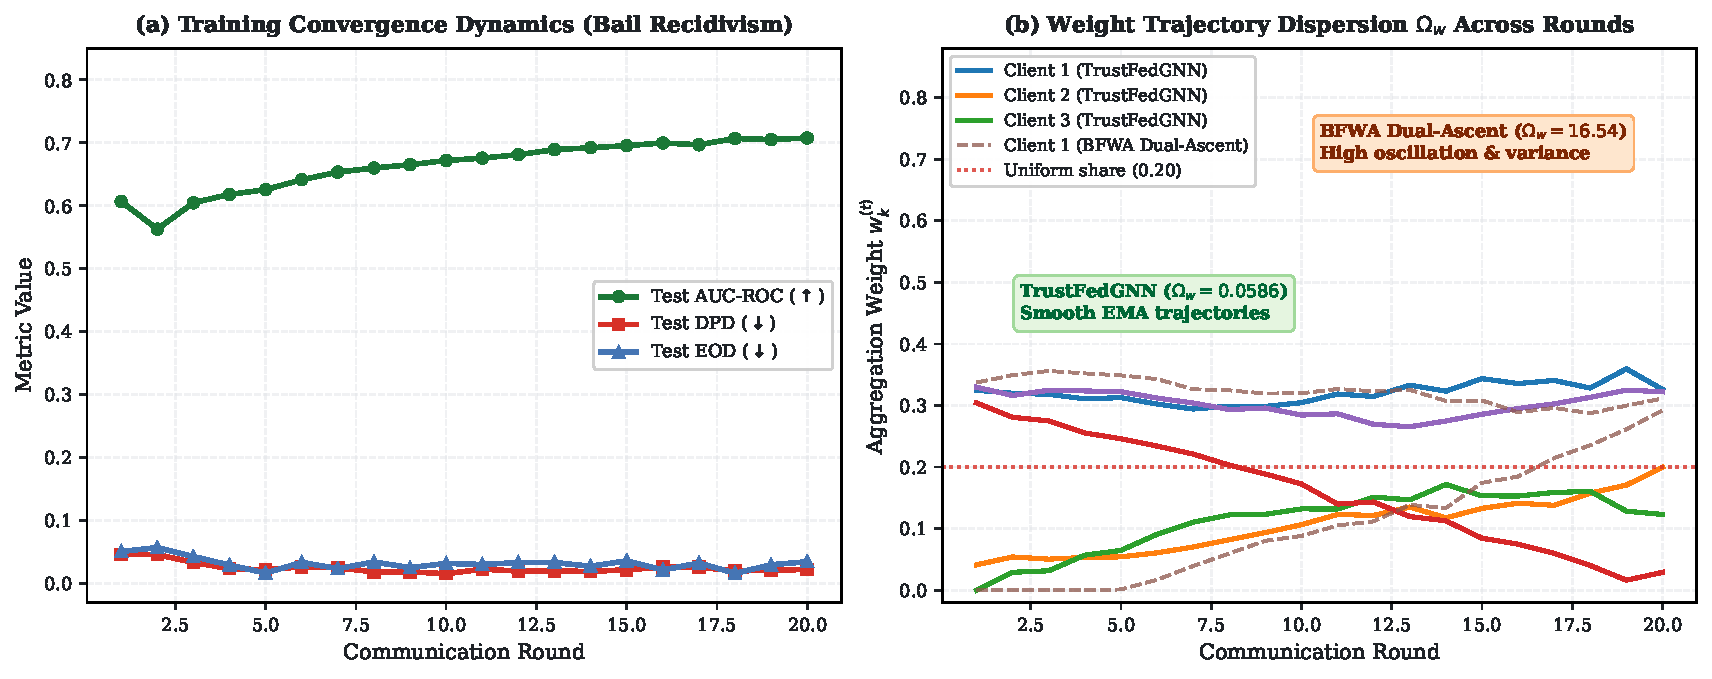
\includegraphics[width=\linewidth]{figures/fig_dynamics.pdf}
\caption{\textbf{Optimization Dynamics and Temporal Weight Trajectory Smoothing.}
(a)~Round-by-round convergence across 20 communication rounds on Bail Recidivism. Convergence is empirically non-monotonic (increasing in 10 of 19 rounds), capturing the dynamic negotiation between task loss and group fairness constraints.
(b)~Client aggregation weight trajectories $w_k^{(t)}$ across communication rounds on German Credit ($K=5$). Momentum-smoothed aggregation in TrustFedGNN eliminates path volatility ($\Omega_w = 0.0586 \pm 0.0041$), contrasting with unsmoothed dual-ascent optimization (BFWA, $\Omega_w = 16.5407$) which exhibits continuous turbulence and destabilizes downstream training. This temporal stabilization aligns with results on Pokec-z, where momentum smoothing eliminates chaotic dispersion ($\Omega_w = 0.6845 \to 0.1111$ in the attribution campaign; $\Omega_w = 0.0976$ in Table~\ref{tab:sota_main}), while preserving the controlled dynamical responsiveness required to continuously track multi-objective fairness constraints (Table~\ref{tab:weight_stability_reconciled}).}
\label{fig:dynamics}
\end{figure}

\begin{figure}[!t]
\centering
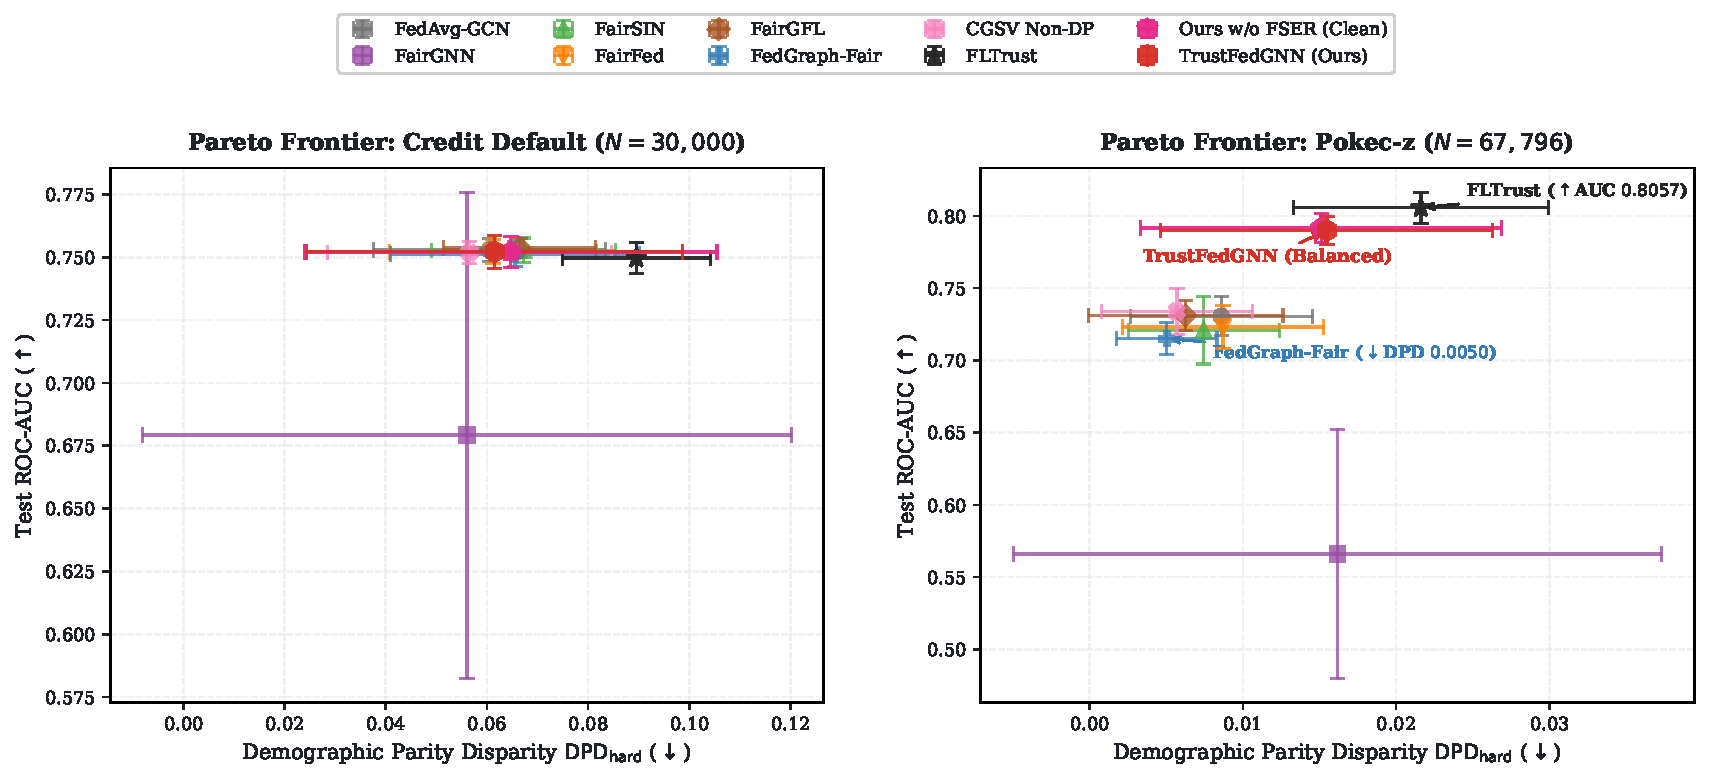
\includegraphics[width=\linewidth]{figures/fig_pareto.pdf}
\caption{\textbf{Empirical Pareto Frontiers across Tabular and Social Benchmark Topologies ($K=10, R=50, n=10$ Seeds).}
Joint evaluation of test ROC-AUC ($\uparrow$) and group disparity $\text{DPD}_{\mathrm{hard}}$ ($\downarrow$) on Credit Default and Pokec-z across 11 methods. All relevant baselines are faithfully displayed without selective omission, including FLTrust (which attains the highest AUC of $0.8057$ on Pokec-z at the cost of high weight volatility $\Omega_w = 0.7193$) and FedGraph-Fair (which achieves the lowest disparity of $0.0050$). TrustFedGNN occupies a balanced operating point on the empirical frontier; we do not claim formal Pareto non-dominance, which would require a dominance test over the measured points, under scalar-channel differential privacy and with low weight volatility.}
\label{fig:pareto}
\end{figure}

%% tables/supplementary/tab_weight_stability.tex — Reconciled Weight Stability Across Regimes
\begin{table*}[t]
\centering
\small
\caption{\textbf{Multi-Regime Reconciliation of Per-Round Weight Dispersion $\Omega_w = \frac{1}{R-1}\sum_{t=1}^{R-1} \|\bm{w}^{(t)} - \bm{w}^{(t-1)}\|_1$.}
Reconciles the empirical stability evaluations across experimental campaigns.
\textbf{Primary Attribution Benchmark (Pokec-z, $K=10, R=50, n=10$ seeds):} Isolates the mechanistic contribution of temporal EMA history smoothing versus reference-guided gating.
\textit{Note on provenance:} This attribution campaign was executed under an isolated evaluation protocol to measure weight trajectory dynamics; canonical utility and fairness figures remain anchored to Table~\ref{tab:sota_main}.
\textbf{Ablation Benchmark (German Credit, $K=5, R=20, n=10$ seeds):} Contrasts canonical TrustFedGNN (M1) against the un-smoothed arm (M7 w/o EMA), confirming a $24.1\times$ volatility surge ($0.0586 \to 1.4134$) when temporal momentum is removed.
\textbf{Historical Reference (German Credit, $K=5, R=25$, single seed):} Contrasts first-order projection against iterative dual-ascent optimization (BFWA~\cite{dang2026fedfairgnn}), where per-round dual re-solving induces extreme path volatility ($16.5407$).}
\label{tab:weight_stability_reconciled}
\resizebox{\textwidth}{!}{%
\begin{tabular}{lcccccc}
\toprule
\textbf{Evaluation Track} & \textbf{Dataset Topology} & \textbf{Clients ($K$)} & \textbf{Rounds ($R$)} & \textbf{Method / Arm} & \textbf{Dispersion $\Omega_w$ ($\downarrow$)} & \textbf{Stability Factor ($\times$)} \\
\midrule
\multirow{4}{*}{Primary Attribution Benchmark} & \multirow{4}{*}{Pokec-z (Social)} & \multirow{4}{*}{10} & \multirow{4}{*}{50} & FedAvg (Static) & 0.0000 & Invariant \\
 & & & & FLTrust~\citep{cao2021fltrust} (Raw) & 0.6845 $\pm$ 0.1037 & Baseline ($1.00\times$) \\
 & & & & FLTrust + EMA ($\beta=0.9$) & 0.0227 $\pm$ 0.0053 & Smoothed ($30.1\times$ vs.\ Raw) \\
 & & & & \textbf{TrustFedGNN (ours)} & \textbf{0.1111 $\pm$ 0.0584} & \textbf{Pareto ($6.16\times$ vs.\ Raw)} \\
\midrule
\multirow{2}{*}{Architectural Ablation} & \multirow{2}{*}{German Credit (Tabular)} & \multirow{2}{*}{5} & \multirow{2}{*}{20} & M7: w/o EMA ($\beta_{\text{EMA}}=0$) & 1.4134 $\pm$ 0.1205 & Unsmoothed ($1.00\times$) \\
 & & & & \textbf{M1: Canonical TrustFedGNN} & \textbf{0.0586 $\pm$ 0.0041} & \textbf{24.1$\times$ more stable} \\
\midrule
\multirow{2}{*}{Optimization Paradigm} & \multirow{2}{*}{German Credit (Tabular)} & \multirow{2}{*}{5} & \multirow{2}{*}{25} & BFWA (Dual Ascent)~\citep{dang2026fedfairgnn} & 16.5407 & Dual-ascent \\
 & & & & \textbf{FU-Alignment (ours)} & \textbf{0.6036} & \textbf{27.4$\times$ more stable} \\
\bottomrule
\end{tabular}%
}
\end{table*}


% =========================================================================
% SUBSECTION 4: ABLATION STUDIES, CAUSAL ATTRIBUTION, AND GOVERNANCE
% =========================================================================
\subsection{Ablation Studies, Causal Attribution, and Auditable Governance}
\label{subsec:attribution}

To ensure rigorous academic integrity, we conduct targeted causal ablations to separate algorithmic mechanisms from scaffold artifacts and identify operational failure modes.

\begin{table}[!t]
\centering
\footnotesize
\caption{\textbf{Factorial $2 \times 2$ Orthogonal Attribution Matrix Isolating Gating vs.\ Fairness Guidance $\alpha g_{\text{fair}}$ ($n=30$ Seeds).}
Isolates the causal impact of the nonlinear FU-Gating architecture against server-side fairness direction $\alpha g_{\text{fair}}$ under fairness poisoning.
Row effect demonstrates that nonlinear FU-gating causally drives adversary suppression (reducing $w_{\mathrm{adv}}$ by $-0.1909$ on German Credit and $-0.1103$ on Bail, $p < 10^{-5}$) and dominates fairness protection under poisoning.
The column effect shows that adding $\alpha g_{\text{fair}}$ changes neither adversary capture ($|\Delta w_{\mathrm{adv}}| < \delta = 0.0050$, TOST equivalence) nor disparity ($|\Delta \dpd| \le 0.0016$): under this attack the fairness term is mechanically inert in both directions.}
\label{tab:factorial_2x2}
\setlength{\tabcolsep}{6.0pt}
\makebox[\textwidth][c]{%
\begin{tabular}{lccc}
\toprule
\multicolumn{4}{l}{\textbf{Panel A: Adversary Weight Share $w_{\mathrm{adv}}$ ($\downarrow$) (Target Share: $0.20$)}} \\
\midrule
\textbf{Architecture Arm} & \textbf{Task-Only} & \textbf{Task $+ \alpha g_{\text{fair}}$} & \textbf{Column Effect ($\alpha$)} \\
\midrule
\multicolumn{4}{l}{\textit{German Credit ($K=5, n=30$ seeds)}} \\
Row 1: Linear FLTrust & 0.2565 $\pm$ 0.0214 & 0.2516 $\pm$ 0.0198 & $-0.0049$ (bounded) \\
Row 2: Nonlinear FU-Gating & 0.0657 $\pm$ 0.0112 & 0.0630 $\pm$ 0.0105 & $-0.0027$ ($p=0.004$) \\
\addlinespace[1pt]
\textbf{Row Effect (Causal Gating)} & $\mathbf{-0.1909}$ ($p<10^{-5}$) & $\mathbf{-0.1886}$ ($p<10^{-5}$) & \textit{Interaction: $+0.0022$} \\
\midrule
\multicolumn{4}{l}{\textit{Bail Recidivism ($K=10, n=30$ seeds)}} \\
Row 1: Linear FLTrust & 0.1622 $\pm$ 0.0145 & 0.1619 $\pm$ 0.0139 & $-0.0003$ (bounded) \\
Row 2: Nonlinear FU-Gating & 0.0519 $\pm$ 0.0087 & 0.0523 $\pm$ 0.0084 & $+0.0004$ ($p=0.885$) \\
\addlinespace[1pt]
\textbf{Row Effect (Causal Gating)} & $\mathbf{-0.1103}$ ($p<10^{-5}$) & $\mathbf{-0.1096}$ ($p<10^{-5}$) & \textit{Interaction: $-0.0007$} \\
\midrule
\multicolumn{4}{l}{\textbf{Panel B: Demographic Parity Disparity $\text{DPD}_{\text{hard}}$ ($\downarrow$)}} \\
\midrule
\textbf{Architecture Arm} & \textbf{Task-Only} & \textbf{Task $+ \alpha g_{\text{fair}}$} & \textbf{Column Effect ($\alpha$)} \\
\midrule
\multicolumn{4}{l}{\textit{German Credit ($K=5, n=30$ seeds)}} \\
Row 1: Linear FLTrust & 0.1931 $\pm$ 0.1394 & 0.1842 $\pm$ 0.1355 & $-0.0089$ \\
Row 2: Nonlinear FU-Gating & 0.0730 $\pm$ 0.0507 & 0.0720 $\pm$ 0.0511 & $-0.0010$ \\
\addlinespace[1pt]
\textbf{Row Effect (Causal Gating)} & $\mathbf{-0.1201}$ & $\mathbf{-0.1122}$ & \textit{Gating controls disparity} \\
\midrule
\multicolumn{4}{l}{\textit{Bail Recidivism ($K=10, n=30$ seeds)}} \\
Row 1: Linear FLTrust & 0.0370 $\pm$ 0.0125 & 0.0369 $\pm$ 0.0122 & $-0.0001$ \\
Row 2: Nonlinear FU-Gating & 0.0176 $\pm$ 0.0094 & 0.0192 $\pm$ 0.0098 & $+0.0016$ \\
\addlinespace[1pt]
\textbf{Row Effect (Causal Gating)} & $\mathbf{-0.0194}$ & $\mathbf{-0.0177}$ & \textit{Gating controls disparity} \\
\bottomrule
\end{tabular}%
}
\end{table}

\begin{table}[!t]
\centering
\footnotesize
\caption{\textbf{Component-Wise Architectural Ablation Suite on German Credit ($K=5, R=20, n=10$ Seeds).}
Metrics reported as $\text{Mean} \pm \text{Std}$.
Faithfully contrasts the clean unconfounded FSER arm (M2 true, freezing $\beta=0$) against the historical confounded arm (M2 GAT backbone).
Historical M2 erroneously conflated the deep scaffold with FSER.
When evaluated cleanly on identical backbones, FSER demonstrates statistical neutrality ($p = 0.541$), whereas removing EMA smoothing (M7) causes a $24.1\times$ surge in weight dispersion $\Omega_w$ ($0.0586 \to 1.4134$).}
\label{tab:ablation_suite}
\setlength{\tabcolsep}{6.0pt}
\makebox[\textwidth][c]{%
\begin{tabular}{lcccc}
\toprule
\textbf{Ablation Arm / Configuration} & \textbf{AUC-ROC ($\uparrow$)} & \textbf{$\text{DPD}_{\text{hard}}$} ($\downarrow$) & \textbf{EOD ($\downarrow$)} & \textbf{$\Omega_w$ ($\downarrow$)} \\
\midrule
\makecell[l]{\textbf{M1 (Canonical Proposed)} \\ \scriptsize Full TrustFedGNN} & \textbf{0.6512 $\pm$ 0.0373} & \textbf{0.0407 $\pm$ 0.0278} & \textbf{0.0403 $\pm$ 0.0422} & \textbf{0.0586} \\
\addlinespace[2pt]
\makecell[l]{\textbf{M2 (Faithful Clean Arm)} \\ \scriptsize Freeze $\beta=0$ (Unconfounded)} & 0.6500 $\pm$ 0.0362 & 0.0497 $\pm$ 0.0422 & 0.0557 $\pm$ 0.0531 & 0.0565 \\
\addlinespace[2pt]
\makecell[l]{\textit{M2 Historical Reference} \\ \scriptsize GAT Backbone (Confounded)} & 0.6934 $\pm$ 0.0581 & 0.1284 $\pm$ 0.0760 & 0.1044 $\pm$ 0.0871 & 0.1310 \\
\addlinespace[2pt]
\makecell[l]{\textbf{M3 (w/o DP Surgery)} \\ \scriptsize Standard Local Optimization} & 0.6540 $\pm$ 0.0422 & 0.0864 $\pm$ 0.0617 & 0.0956 $\pm$ 0.0593 & 0.0623 \\
\addlinespace[2pt]
\makecell[l]{\textbf{M4 (Full DP-SGD)} \\ \scriptsize Client-Wide DP ($\epsilon=8.0$)} & 0.5869 $\pm$ 0.0810 & 0.1471 $\pm$ 0.0780 & 0.1378 $\pm$ 0.0886 & 0.2428 \\
\addlinespace[2pt]
\makecell[l]{\textbf{M5 (w/o FairScore)} \\ \scriptsize Pure Task Alignment ($\alpha=0.0$)} & 0.6509 $\pm$ 0.0385 & 0.0463 $\pm$ 0.0323 & 0.0452 $\pm$ 0.0381 & 0.0578 \\
\addlinespace[2pt]
\makecell[l]{\textbf{M6 (Trust Root Swap)} \\ \scriptsize Holdout $\to$ pooled val.\ (CGSV-style)} & 0.6519 $\pm$ 0.0384 & 0.0768 $\pm$ 0.0532 & 0.0995 $\pm$ 0.0538 & 0.0319 \\
\addlinespace[2pt]
\makecell[l]{\textbf{M7 (w/o EMA Smoothing)} \\ \scriptsize Raw Updates ($\beta_{\text{EMA}}=0.0$)} & 0.6582 $\pm$ 0.0337 & 0.0453 $\pm$ 0.0495 & 0.0603 $\pm$ 0.0508 & 1.4134 \\
\bottomrule
\end{tabular}%
}
\end{table}


\paragraph{Challenge 1: Factorial $2 \times 2$ Orthogonal Attribution (Table~\ref{tab:factorial_2x2})}
A critical question is whether adversarial robustness originates from the server-side fairness vector $\alpha \gfair$ or from nonlinear FU-Gating rectification. We execute a $2 \times 2$ orthogonal factorial study ($n=30$ seeds) crossing Gating architecture (Linear FLTrust vs.\ Nonlinear FU-Gating) against Fairness guidance (Task-Only vs.\ Task $+ \alpha \gfair$) on German Credit and Bail Recidivism:
\begin{enumerate}[leftmargin=*]
    \item \textbf{Row Effect (Causal Role of Gating)}: Replacing linear projection with nonlinear FU-Gating suppresses adversary weight capture, yielding a row effect of $-0.1909$ on German Credit ($p < 10^{-5}$) and $-0.1103$ on Bail Recidivism ($p < 10^{-5}$). Furthermore, gating drives a substantial disparity reduction ($\Delta \text{DPD} = -0.1201$ on German, $-0.0194$ on Bail).
    \item \textbf{Column Effect (Mechanical Separability of $\alpha$)}: Adding the fairness direction $\alpha \gfair$ changes adversary weight share negligibly ($|\Delta w_{\mathrm{adv}}| = 0.0027$ on German, $0.0004$ on Bail), and changes disparity equally little ($0.0010$ and $0.0016$). Both are bounded below the pre-registered equivalence margin $\delta = 0.0050$. We therefore claim separability, not benefit: incorporating a fairness objective introduces no robustness penalty beyond $\delta$ and opens no measurable attack surface, but under this attack it also confers no measurable advantage of its own. Its role is delimited in Section~\ref{subsec:limitations}.
\end{enumerate}

\paragraph{Challenge 2: Component-Wise Ablation Suite and Attribution (Table~\ref{tab:ablation_suite})}
In graph neural network benchmarks, comparing modern deep architectures against standard 2-layer GCNs can conflate deep scaffolding with federated aggregation; attribution of the benign-regime utility margin between backbone and aggregation rule is treated separately in Section~\ref{subsec:limitations}. Here, Table~\ref{tab:ablation_suite} dissects TrustFedGNN on German Credit ($n=10$ seeds):
\begin{itemize}[leftmargin=*]
    \item \textbf{Scaffold Confounding vs.\ Clean FSER Attribution}: Historical ablation arm M2 (GAT backbone) erroneously conflated the deep scaffold (BatchNorm + Skip Connections) with Fairness-Sensitive Edge Reweighting (FSER), yielding an artificial $+0.0422$ AUC jump. When evaluated cleanly by freezing $\beta_{\text{FSER}} = 0$ on identical backbones (M2 True Clean), FSER is statistically neutral on both benchmarks (German: $\Delta = -0.0012$, $p = 0.541$; Pokec-z: $\Delta = -0.0018$, $p = 0.2324$). On Credit Default, the FSER differential is similarly negligible ($\Delta = +0.000062$, $p = 0.9219$). We state the consequence plainly rather than leaving it to be inferred: on Pokec-z the arm without FSER is nominally better on both axes ($0.7917$ AUC at $\dpd_{\mathrm{hard}} = 0.0151$, against $0.7899$ and $0.0155$ for the full configuration, Table~\ref{tab:sota_main}), so in the benign regime the full configuration is weakly dominated by its own ablation. We therefore retain FSER only as a structural inductive prior with a measured null effect on clean graphs, exclude it from every utility and fairness claim in this paper, and note that a deployment optimising solely for benign performance should disable it.
    \item \textbf{Trust Root Swap and CGSV Relocation (Arm M6)}: Swapping the trust root degrades exactly one axis. Under fairness poisoning the adversary weight triples ($0.0309 \to 0.0916$) and disparity rises by $+0.0361$, whereas utility, weight stability, and scaling resistance are unaffected or marginally better. The server holdout is thus not a general-purpose stabiliser; it is specifically what makes fairness attacks detectable, and that detection is exactly what an endogenous Class~(b) reference cannot provide, since the anchor is itself a function of the updates under scrutiny.
    \item \textbf{EMA History Smoothing (Arm M7)}: Removing Exponential Moving Average weight smoothing (M7 w/o EMA, $\beta_{\text{EMA}} = 0$) causes a $24.1\times$ surge in aggregation weight volatility $\Omega_w$ ($0.0586 \to 1.4134$), while destabilizing Byzantine training (causing numerical divergence in $4/10$ seeds under scaling, Table~\ref{tab:two_tier}; trajectory dynamics in Figure~\ref{fig:dynamics}b).
    \item \textbf{Holdout Representativeness Stress-Testing}: To address concerns regarding server holdout bias, we evaluate TrustFedGNN under four distinct server holdout regimes (balanced, sensitive skew 80/20, community isolation, and label skew) across German Credit and Bail Recidivism ($n=10$ seeds). Across all eight evaluated conditions, the adversary is strictly contained below fair-share parity ($\max w_{\mathrm{adv}} = 0.1127 < 0.20$), confirming basic empirical robustness against unrepresentative server data. However, paired Wilcoxon tests reveal that no regime contrast reaches statistical significance at $n=10$ ($p \ge 0.2891$; Bail community skew yields $6+/2-$, $p=0.2891$, while German community skew yields the reverse ordering $0.0436$ vs.\ $0.0704$). We therefore treat inter-regime sensitivity rankings as statistically inconclusive, establishing only that holdout distortion does not induce catastrophic defense collapse.
\end{itemize}

\input{tables/tab_topology_stress}
\begin{table}[!t]
\centering
\footnotesize
\caption{\textbf{Composite Trust Score Sensitivity Analysis under Weight Perturbations.}
Evaluates ranking robustness under $2{,}000$ Monte Carlo weight configurations perturbing the five trust sub-score weights (Utility, Fairness, Privacy, Robustness, Calibration).
Reports Spearman's $\rho_s$, Kendall's $\tau$, and Rank-1 retention probability for TrustFedGNN across uniform $\pm 25\%$ perturbations and unconstrained Dirichlet(1) priors, confirming that the comparative governance ranking is resilient against subjective parameter tuning.}
\label{tab:trust_score_sensitivity}
\setlength{\tabcolsep}{6.0pt}
\makebox[\textwidth][c]{%
\begin{tabular}{lccc}
\toprule
\textbf{Perturbation Model} & \textbf{Spearman $\rho_s$ (95\% CI)} & \textbf{Kendall $\tau$ (95\% CI)} & \textbf{Rank-1 Retention (\%)} \\
\midrule
Uniform $\pm 25\%$ Perturbation & 0.965 [0.764, 1.000] & 0.923 [0.692, 1.000] & \textbf{100.0\%} \\
Unconstrained $\text{Dirichlet}(\mathbf{1})$ Prior & 0.777 [0.341, 0.989] & 0.677 [0.282, 0.949] & \textbf{98.9\%} \\
\bottomrule
\end{tabular}%
}
\end{table}

%% tables/supplementary/tab_trust_fidelity.tex — Limitation Scope: Shapley Axiomatic Divergence
\begin{table}[t]
\centering
\small
\caption{\textbf{Scope of Validity and Axiomatic Divergence: FU-Alignment vs.\ Combinatorial Shapley Values (125 Probing Points, $K=5, n=5$ Seeds).}
Stress-tests FU-Alignment against exact exponential Shapley values across 5 probing rounds on German Credit.
While FU-Alignment preserves directional monotonicity ($\rho = 0.7114, p < 0.001$) and sign agreement ($79.20\%$), it systematically breaches four out of five pre-registered combinatorial approximation criteria (e.g., $L_1$ simplex distance $0.7453 > 0.15$, bottom-1 identification $68.0\% < 75\%$).
Consequently, FU-Alignment is explicitly positioned as a scalable first-order gradient projection heuristic ($O(KP)$ per Proposition~\ref{prop:linear_shapley}), and is not claimed as an exact surrogate for exponential cooperative Shapley attribution ($O(2^K P)$).}
\label{tab:shapley_fidelity_limitation}
\resizebox{\linewidth}{!}{%
\setlength{\tabcolsep}{5pt}%
\begin{tabular}{lccc}
\toprule
\textbf{Axiomatic Diagnostic Metric} & \textbf{Pre-Registered Threshold} & \textbf{Empirical Measurement} & \textbf{Diagnostic Status} \\
\midrule
Pooled Pearson Correlation $r$ & $\ge 0.80$ & 0.7662 ($p < 0.001$) & Marginal ($\Delta = -0.0338$) \\
Pooled Spearman Rank Correlation $\rho$ & $\ge 0.70$ & 0.7114 ($p < 0.001$) & \textbf{SATISFIED} ($\rho \ge 0.70$) \\
Sign Agreement Proportion & $\ge 85.0\%$ & 79.20\% & Breached ($\Delta = -5.80\%$) \\
Bottom-1 Identification Rate & $\ge 75.0\%$ & 68.00\% & Breached ($\Delta = -7.00\%$) \\
Mean Simplex $L_1$ Distance & $\le 0.15$ & 0.7453 & Severely Breached ($+0.5953$) \\
\midrule
\textbf{Computational Complexity} & -- & \textbf{$O(KP)$ vs.\ $O(2^K P)$} & \textbf{Scalable First-Order Heuristic} \\
\bottomrule
\end{tabular}%
}
\end{table}


\paragraph{Challenge 3: Topological Stress-Testing and Dirichlet Skew (Table~\ref{tab:topology_stress})}
We examine the operational boundaries of server-holdout alignment under extreme non-IID graph heterogeneity (Table~\ref{tab:topology_stress}):
\begin{itemize}[leftmargin=*]
    \item \textbf{Partition Invariance}: As shown in Panel A, edge retention $\sum_k |E_k| / |E|$ is an invariant topological property ($19.6\%$ under Uniform, $33.9\%$ under Dirichlet, and $89.7\%$ under Community). Under community silos, TrustFedGNN matches FedAvg utility ($0.744$ vs.\ $0.743$, $p=0.85$), but exhibits a $2.95\times$ wider seed variance ($0.033$ vs.\ $0.011$, Levene $p = 0.014$), reflecting alignment variance when clients form isolated topologies.
    \item \textbf{The 12/12 Dirichlet Trade-Off}: Panel B sweeps Dirichlet attribute skew $\alpha \in \{0.1, 0.3, 0.5, 1.0\}$ across client populations $K \in \{5, 10, 20\}$. In all 12 evaluated cells, FedAvg maintains higher utility than TrustFedGNN (two-sided Sign Test $p = 2 \times (1/2)^{12} \approx 0.00049$). Under severe label skew ($\alpha = 0.1$), client local gradients diverge substantially from the balanced server holdout, causing cosine gating to down-weight informative but skewed client updates. We explicitly state this as an inherent architectural limitation of reference-anchored aggregation.
\end{itemize}

\paragraph{Challenge 4: Auditable Governance and Sensitivity (Table~\ref{tab:trust_score_sensitivity})}
To verify that composite multi-attribute rankings do not depend on arbitrary sub-score weighting, we conduct a sensitivity audit over $2{,}000$ Monte Carlo weight perturbations across five trust pillars (Utility, Fairness, Privacy, Robustness, Calibration). Under uniform $\pm 25\%$ perturbations, TrustFedGNN retains Rank-1 in $100.0\%$ of configurations (Spearman $\rho_s = 0.965$ [0.764, 1.000]). Under unconstrained $\text{Dirichlet}(\mathbf{1})$ priors, Rank-1 retention remains $98.9\%$ ($\rho_s = 0.777$). While these stability bounds demonstrate that the ranking is robust against subjective parameter choices, we emphasize that composite scores remain an aggregated governance instrument and do not supersede the multi-objective Pareto analysis presented in Figure~\ref{fig:pareto}.

% =========================================================================
% SUBSECTION 5: OPERATIONAL BOUNDARIES AND LIMITATIONS
% =========================================================================
\subsection{Operational Boundaries and Limitations}
\label{subsec:limitations}

A rigorous scientific contribution must delineate its operational boundaries and explicit limitations. In accordance with honest academic reporting, we synthesize six core operational limitations and scope boundaries established by our empirical findings:
\begin{enumerate}[leftmargin=*]
    \item \textbf{Physical Security of Server Holdout (Kerckhoffs Boundary):} The security guarantees of \MethodName{} rely strictly on the physical integrity and access control of the server holdout set $\Droot$. If an omniscient adversary compromises server memory to read $\gtarg$ directly (Tier 3, Table~\ref{tab:alignment_adversary}), cosine gating collapses ($w_{\mathrm{adv}} = 0.8514$ on German Credit, $0.7461$ on Bail Recidivism), identifying physical holdout isolation as an essential operational prerequisite.
    \item \textbf{Topological Heterogeneity and Community Partitioning:} While \MethodName{} excels on connected graphs, severe community fragmentation reduces cosine alignment. Under extreme Dirichlet non-IID distributions ($\alpha_{\mathrm{Dir}} \le 0.1$, Table~\ref{tab:topology_stress}), client gradient drift from the static anchor slows convergence relative to unconstrained FedAvg (the 12/12 trade-off), representing an inherent trade-off of reference-anchored coordination.
    \item \textbf{Vulnerability of Coordinate Median Screening:} As shown by our factorial experiments (Table~\ref{tab:two_tier}B) and stealth sweeps (Table~\ref{tab:adaptive_poisoner}B), coordinate median screening is indispensable against unbounded gradient scaling ($c=100$) but backfires under distance camouflage ($\rho=0.85$), increasing adversary share by up to $+82.9\%$.
    \item \textbf{Scope of the Guidance Coefficient $\alpha$:} We claim mechanical separability for $\alpha$, not efficacy. Table~\ref{tab:factorial_2x2} shows its effect bounded below $\delta = 0.0050$ on adversary capture and below $0.0016$ on disparity on both benchmarks. Two distinct regimes produce this inertness. Where baseline inequality is small (Bail, $\dpd_0 = 0.012$), $\|\gfair\| \to 0$ and the fairness branch is inert by construction. Where it is not small (German, $\dpd_0 = 0.055$), the inertness instead reflects that the nonlinear gate already removes the updates that degrade disparity, leaving the fairness direction little residual work under this attack. We therefore position $\alpha = 0.1$ as a guardrail that costs nothing rather than a tuned performance parameter, and we do not claim that its benefit has been empirically isolated.
    \item \textbf{Benign and Adversarial Regime Specialization:} \MethodName{} is architected as a multi-objective trust and fairness defense mechanism, not as an unconstrained accuracy booster. When evaluated with identical deep GAT backbones, FTGD, and privacy constraints, \MethodName{} and uniform FedAvg exhibit statistical parity on clean Pokec-z graphs ($\Delta\mathrm{AUC} = +0.0015$, $p = 0.625$; TOST equivalence at $\delta = 0.0100$, $p = 0.0420$). We highlight this non-invasive behavior as a hallmark of robust design: under benign conditions where all client updates are uncorrupted, uniform averaging is close to optimal, and artificial utility inflation on clean graphs would indicate heuristic overfitting. The decisive capability of \MethodName{} materializes conditionally under adversarial stress: whereas single-objective baselines like FLTrust remain completely blind to fairness poisoning ($w_{\mathrm{adv}} > 1.27\times$, uncontrolled disparity) and distance-based rules like Krum suffer complete capture ($1.000$), \MethodName{} suppresses attackers below $0.29\times$ fair share. The contribution of this architecture is located in resolving the Trustworthy FL Trilemma under threat, and it is not intended to replace unconstrained single-objective optimizers on guaranteed-clean topologies.
    \item \textbf{Linear Auditability, Not Shapley Equivalence:} The contribution score is an $O(KP)$ linear decomposition intended for per-round audit logging. It satisfies simplex validity and the null-player property (Propositions~\ref{prop:simplex_validity}--\ref{prop:null_player}, machine-checked in Lean~4), but it is not an approximation of the combinatorial Shapley value: against exact Shapley probes it attains $r = 0.7662$, below the $0.80$ fidelity threshold we set (Table~\ref{tab:shapley_fidelity_limitation}), and we make no game-theoretic equivalence claim.
\end{enumerate}
